\documentclass[uplatex,dvipdfmx]{jsarticle}
\usepackage{url}
\usepackage{longtable}
\usepackage{tabularx}
\usepackage{array}
\usepackage{multirow}
\usepackage{amsmath}
\usepackage{amssymb}
\usepackage{graphicx}
\usepackage{tikz}
\usetikzlibrary{shapes.geometric, arrows.meta, positioning, fit, backgrounds}
\usepackage{pgfplots}
\pgfplotsset{compat=1.18}
\usepackage{algorithm}
\usepackage{algorithmic}
% 図表が入りきらずページ下部が大きく空くのを防ぐ。
% 本文の占有率の下限を下げ、1ページに置ける図表数を増やす。
\renewcommand{\topfraction}{0.9}
\renewcommand{\bottomfraction}{0.85}
\renewcommand{\textfraction}{0.06}
\renewcommand{\floatpagefraction}{0.75}
\setcounter{topnumber}{3}
\setcounter{bottomnumber}{2}
\setcounter{totalnumber}{5}
% 第4章の小節をまとめた際に生じる第4階層の見出しにも番号を付ける。
\setcounter{secnumdepth}{4}
% longtable のキャプション区切りを、通常の表と同じ全角空白へそろえる。
\makeatletter
\def\LT@makecaption#1#2#3{%
  \LT@mcol\LT@cols c{\hbox to\z@{\hss\parbox[t]\LTcapwidth{%
    \sbox\@tempboxa{#1{#2\hskip1zw}#3}%
    \ifdim\wd\@tempboxa>\hsize
      #1{#2\hskip1zw}#3%
    \else
      \hbox to\hsize{\hfil\box\@tempboxa\hfil}%
    \fi
    \endgraf\vskip\baselineskip}%
  \hss}}}
\makeatother
\floatname{algorithm}{アルゴリズム}
\renewcommand{\algorithmicrequire}{\textbf{入力:}}
\renewcommand{\algorithmicensure}{\textbf{出力:}}
% 脚注番号を上付き数字（例：である1。）で示す。
\renewcommand{\thefootnote}{\arabic{footnote}}
\InputIfFileExists{git_revision.tex}{}{%
  \newcommand{\ReportGitCommit}{未設定}%
  \newcommand{\ReportGitTag}{未設定}%
}
\AtBeginDvi{%
  % IPAex TrueTypeをUnicodeで埋め込み、閲覧環境に依存しない日本語表示と
  % 検索・コピーを可能にする（TeX Liveのipaexパッケージを使用）。
  \special{pdf:mapline uprml-h unicode ipaexm.ttf}%
  \special{pdf:mapline uprml-hq unicode ipaexm.ttf}%
  \special{pdf:mapline uprml-v unicode ipaexm.ttf -w 1}%
  \special{pdf:mapline upgbm-h unicode ipaexg.ttf}%
  \special{pdf:mapline upgbm-hq unicode ipaexg.ttf}%
  \special{pdf:mapline upgbm-v unicode ipaexg.ttf -w 1}%
  \special{pdf:tounicode UTF8-UTF16}%
}

\begin{document}

\pagestyle{empty}

\begin{center}
\vspace*{1cm}
\large
{\LARGE 卒業研究報告書}\\
\vspace*{0.8cm}
題目\\
\vspace*{1cm}
\parbox{15.5cm}{\centering\LARGE
収集画像から生成したRTI・部分画像を用いた\\[2mm]
マルチモーダルLLMによるPTP包装識別}\\
\vspace{3mm}

\vspace*{3cm}
指導教員\\
\vspace*{0.3cm}
\underline{\LARGE 森山　真光　准教授}\\
\vspace*{3cm}
報告者\\
\vspace*{0.3cm}

{23--1--211--0009}\\
\vspace*{0.3cm}
\underline{\Huge 呉竹　櫂人}\\
\vspace*{0.5cm}
近畿大学情報学部情報学科\\
\vspace*{2cm}
令和8年10月6日提出\\
\end{center}

\newpage
\normalsize


\clearpage
\begin{center}
{\bf \Large 概要}
\end{center}

薬剤の取り違えは，患者の健康被害につながるおそれがある．PTP包装を画像から識別する従来研究には，1薬剤あたり表裏各72枚を撮影する方法がある．本研究では，各薬剤の表裏各1枚の収集画像から，全体画像，表裏を結合したRTI，部分画像を作る．それらの組合せと画像拡張を変え，視覚言語モデルをLoRAで追加学習する．目的は，少ない元画像から，実写画像の薬剤名を識別することである．

主結果の条件ではRTIを学習に含めず，全体画像と部分画像を用いた．41薬剤の実写287枚に対し，3回の学習の平均正解率は99.54\%，標本標準偏差は0.53ポイントであった．各回の正解数は287枚中286枚，287枚中287枚，287枚中284枚であった．これらの画像は，このモデルの学習には使わなかった．ただし，同じ画像で8条件を比較した後に平均正解率が最も高かった条件を選んだため，結果を見て条件を選んだ影響は残った．

同じ画像と同じ短文プロンプトを与えたGemini 3.8 Flashは，287枚中238枚に正解した．提案手法は学習の3回とも有意に高い正解率を示した．一方，41薬剤の候補一覧を与えたGeminiの283枚とは有意差がなかった．この結果から，今回の41薬剤では，少ない元画像で学習したモデルによって実写を識別する目的をおおむね達成した．

複数薬剤については，実写から作った合成画像800枚を評価した．主結果のモデルでは，最大10候補にすべての正解薬剤が含まれた画像は，3回とも790枚であった．正解の薬剤数だけ候補を残す方式では，平均正解率は85.00\%であった．未知薬剤への回答を保留する仕組みは別の2条件で評価したが，未知58枚中4枚と2枚で誤回答が残った．また，学習薬剤数を100まで増やしても，評価したのは既知41薬剤であり，100薬剤全体の識別性能は確認しなかった．

本手法は，画像を外部サービスへ送らずに使える点にも意義があると考えた．今後の課題として，学習薬剤数を増やしても正解率を保つことと，部分画像の内容や学習量の効果を分けて確かめることが残った．未知薬剤への回答保留と，実写の複数薬剤画像の識別も課題であった．
\newpage

{\small
\tableofcontents
}
\clearpage
\setcounter{page}{1}
\pagestyle{plain}

%----------------------------------------------------------------------
\section{序論}
%----------------------------------------------------------------------

薬剤の取り違えや用量の誤りは，患者に重い健康被害を与えるおそれがある\cite{who_medication}．
PTP包装を画像から識別する従来研究では，1薬剤あたり表裏各72枚，計144枚を撮影している\cite{han2021blister}．
そこで本研究は，各薬剤の表裏各1枚の収集画像から，実写画像の薬剤名を識別することを目指す．
収集画像から表裏を結合した画像（RTI）と部分画像を作り，画像拡張と視覚言語モデルのLoRA追加学習を組み合わせる．

\subsection{研究背景}

薬剤の取り違えや誤服用は，患者の健康被害につながる．
世界保健機関（World Health Organization：WHO）は，投薬に関連する回避可能な健康被害の削減を国際的な目標としている\cite{who_medication}．
医療現場では，外箱や薬袋がない状態で薬剤を鑑別する場合がある．
この場合，錠剤の形状，刻印，色，PTP（Press Through Package）包装上の印字などを手掛かりとする．
末次らは，AI画像解析錠剤識別システムを持参薬の鑑別に導入し，作業時間の短縮とタスク・シフトの可能性を報告している\cite{suetsugu2026ai}．

\subsection{研究課題と目的}

薬剤画像の認識に関する先行研究は，学習用の薬剤画像データセットを構築して手法を評価している\cite{heo2023pill,usuyama2020epillid}．
HanらのPTP包装識別では，250薬剤について計36,000枚を撮影している．同研究は，時間と人手の制約も挙げている\cite{han2021blister}．
学習画像が不足する場合は，幾何変換や色変換によって学習画像の多様性を高める画像拡張が用いられる\cite{shorten2019augmentation}．
そこで本研究は，1薬剤につきフルシートの表面1枚と裏面1枚を学習元とし，そこから派生画像を生成する構成を検討する．
この構成では，残存錠数や切り出し範囲を変えた学習用写真を個別に撮影する必要がない．
ただし，収集画像の取得から前処理までに要する時間は方式間で比較しておらず，総作業時間の削減量は評価対象としない．

本研究では，次の点を評価する．
\begin{itemize}
  \item 41薬剤の単剤正解率を求める．
  \item LoRAを適用していないQwen3.5-4B，およびGeminiと比較する．
  \item 隙間のない合成複数薬剤画像800枚（固定800枚）を識別する．
  \item 未知薬剤への回答を保留する信頼ゲートを予備的に評価する．
  \item 学習薬剤数を41から100へ増やしたときの，既知41薬剤の正解率を調べる．
\end{itemize}
評価には，41薬剤の実写画像287枚を用いる．
本報告書では，学習条件の比較にも使用したこの287枚を，内部開発評価画像と呼ぶ．
内部開発評価画像は，収集画像から構成したLoRA学習集合には含めていない．
一方，同じ287枚を条件検討に反復使用しており，研究初期の実画像方式では一部を学習にも用いた．
そのため，条件決定後に初めて使用する独立最終評価集合ではない．

新しい薬剤への一般化，臨床利用，実写の複数薬剤画像に対する性能，およびRTIと部分画像の個別の寄与は，評価の対象外とする．

\clearpage
\section{関連研究・関連技術}\label{sec:related}
%----------------------------------------------------------------------

\subsection{薬剤画像の認識}

Heoらは，錠剤の刻印，形状，色を認識し，薬剤データベースを検索する手法を提案している\cite{heo2023pill}．
この手法は，刻印検出，外観認識，候補検索など複数の専用モデルを組み合わせる．
Usuyamaらは，約13,000枚から成る公開データセットePillIDを構築している\cite{usuyama2020epillid}．
同ベンチマークでは，大半のクラスで参照画像が片面1枚しかなく，撮影条件の異なる実利用画像を識別する．
Usuyamaらは，メトリクス学習によってこのような少数の参照画像からの識別に取り組んでいる．

これらの研究は，1クラス当たりの参照画像が少ない点で本研究と近い．
一方，識別対象は錠剤本体である．
また，参照画像と照合する方式であるため，識別できるのは参照画像が登録されたクラスに限られる．
本研究は，識別対象をPTP包装とし，収集した表裏画像から派生画像を生成して追加学習する．
さらに，マルチモーダルLLMがクラス名を文字列として生成する点も異なる．

Menahaらは，錠剤や包装の画像を入力し，Google Geminiを用いた薬剤識別支援システムを提案している\cite{menaha2024gemini}．
この手法は外部サービスを用いるプロンプト型であり，本研究は重みを取得可能なモデルを追加学習する点で異なる．

Hanらは，専用の撮影装置を用いてPTP包装の表面と裏面を同時に撮影する手法を提案している\cite{han2021blister}．
向きと大きさを正規化した両面画像であるRTIを作成し，畳み込みニューラルネットワークへ入力して識別する．
本研究は，この両面統合の着想をRTIとして採用する．
ただしHanらは，専用装置による包装全体の撮影を前提とする．
本研究は，専用装置を用いず，部分的なPTP包装画像も対象とする．
また，Hanらは左右結合後の画像を224$\times$224画素に変換して識別器へ入力した．
本研究は，左右結合後の画像を448$\times$448画素へ直接リサイズするため，結合前の縦横比を保持しない．

表\ref{tab:related_comparison}に，関連研究と本研究の相違を示す．
本研究は，収集したPTP包装画像から派生画像を生成し，マルチモーダルLLMを追加学習する点に特徴がある．
また，未知薬剤への対応は予備評価にとどまり，安全な保留を実証したものではない．

\begin{table}[htbp]
  \centering
  \caption{関連研究と本研究の位置付け}
  \label{tab:related_comparison}
  \small
  \renewcommand{\arraystretch}{1.25}
  \setlength{\tabcolsep}{3.5pt}
  \begin{tabularx}{\textwidth}{|>{\raggedright\arraybackslash}p{1.7cm}|>{\raggedright\arraybackslash}p{1.6cm}|>{\raggedright\arraybackslash}X|>{\raggedright\arraybackslash}X|>{\centering\arraybackslash}p{1.3cm}|}
    \hline
    研究 & 対象 & 主な入力 & 手法 & 専用装置 \\ \hline
    Heoら\cite{heo2023pill} & 錠剤 & 錠剤画像 & 刻印・外観認識とデータベース検索 & 不要 \\ \hline
    Usuyamaら\cite{usuyama2020epillid} & 錠剤 & 片面1枚の参照画像と実利用画像 & 画像の特徴の近さを学習する手法 & 不要 \\ \hline
    Menahaら\cite{menaha2024gemini} & 錠剤・包装 & 錠剤・包装画像とプロンプト & 外部サービスのGeminiによる生成 & 不要 \\ \hline
    Hanら\cite{han2021blister} & PTP包装 & 専用装置で撮影した表裏 & RTIとCNN & 必要 \\ \hline
    本研究 & PTP包装 & PTP包装の表裏・部分画像と共通プロンプト & RTI・部分画像とQwen3.5-4B（マルチモーダルLLM）のLoRA追加学習 & 不要 \\ \hline
  \end{tabularx}
\end{table}

\subsection{マルチモーダルLLM}\label{sec:vlm}

画像とテキストを同一モデルで扱うモデルは，視覚言語モデル（Vision-Language Model：VLM）と呼ばれる．
本報告書では，大規模言語モデルを基盤とし，画像とプロンプトを入力して文字列を生成するものをマルチモーダルLLMと呼ぶ．
Baiらは，画像とテキストを統合して扱うQwen-VLを提案している\cite{bai2023qwenvl}．
マルチモーダルLLMは，入力画像を特徴ベクトルの列に変換する視覚エンコーダ，その出力を言語モデルの表現空間へ写像する射影部，および文字列を逐次生成する言語モデルのデコーダから構成される．
この構成により，分類ラベルの番号ではなく薬剤名という文字列を出力できる．
PTP包装では，文字情報と外観情報の双方が識別の手掛かりとなる．
そのため，両者を同一モデルで扱えるマルチモーダルLLMを採用する．

本研究では，Qwen3.5-4Bの特定のリビジョンを用いる\cite{qwen35model}．
入力画像に「この錠剤は何という薬ですか？薬剤名だけで答えてください。」というプロンプトを与え，出力を薬剤クラス名と照合する．

\subsection{LoRA}

LoRA（Low-Rank Adaptation）は，事前学習済みモデルの重みを固定し，低ランク行列だけを追加学習する手法である\cite{hu2022lora}．
元の重み行列を$W_0 \in \mathbb{R}^{d \times k}$とすると，学習後の変換は式\eqref{eq:lora}で表す．

\begin{equation}
  h = \left(W_0 + \frac{\alpha}{r}BA\right)x,
  \quad
  A \in \mathbb{R}^{r \times k},
  \quad
  B \in \mathbb{R}^{d \times r}
  \label{eq:lora}
\end{equation}

ここで，$x \in \mathbb{R}^{k}$は入力，$h \in \mathbb{R}^{d}$は出力，$r$はランク，$\alpha$は更新量の倍率を調整する係数である．
$r$を大きくすると学習可能パラメータ数が増え，$\alpha/r$が元の重みに加える変化の大きさを定める．
本研究で用いる$r$，$\alpha$および学習対象層は，第\ref{sec:method}章と第\ref{sec:results}章で示す．

\subsection{未知入力の保留}

選択的分類は，確信できない入力への回答を保留し，回答率と誤り率を調整する考え方である\cite{geifman2017selective}．
薬剤鑑別では，未知薬剤を既知薬剤として回答すると危険な誤回答になり得る．
本研究では，この考え方に基づく保留機構を信頼ゲートと呼ぶ．
信頼ゲートは，モデル自身の出力だけを信号とする簡単な構成であり，分布外入力の検出手法は適用していない．
そのため，未知薬剤を検出する他の手法との優劣までは扱わない．

%----------------------------------------------------------------------
\clearpage
\section{収集画像からの薬剤名識別と評価方法}\label{sec:method}
%----------------------------------------------------------------------

\subsection{処理の全体像}

図\ref{fig:pipeline}に，提案手法の処理をUMLのアクティビティ図として示す．
図は学習側と評価側の2つの区画に分ける．
学習側では，収集した表裏のPTP包装画像の出典を確認する．次に，背景を除去し，向きと大きさをそろえる．
続いて，RTIと各面の部分画像を作り，各実験条件で定めた画像拡張を適用する．主結果の条件では，RTIを学習に含めず，全体画像と部分画像を用いる．
そのうえで，マルチモーダルLLMをLoRAで追加学習する．
評価側では，学習に使用していない内部開発評価画像を448$\times$448画素へ正規化して入力する．
学習済みLoRAを使って薬剤名を生成し，正解ラベルと照合して正解率を算出する．学習時は画像と共通のプロンプトを入力し，正解薬剤名を回答として与える．識別時は，同じプロンプトと画像を入力し，正解名を与えない．

\begin{figure}[htbp]
  \centering
  \begin{tikzpicture}[
    scale=0.82, transform shape,
    act/.style={
      draw, rounded corners=3mm, align=center, text width=3.9cm,
      minimum height=1.0cm, font=\small, fill=blue!6, inner sep=3pt
    },
    pact/.style={
      draw, rounded corners=3mm, align=center, text width=2.95cm,
      minimum height=1.0cm, font=\small, fill=blue!6, inner sep=3pt
    },
    eact/.style={
      draw, rounded corners=3mm, align=center, text width=3.9cm,
      minimum height=1.0cm, font=\small, fill=orange!8, inner sep=3pt
    },
    bar/.style={draw, fill=black, minimum width=5.0cm, minimum height=1.5mm, inner sep=0pt},
    ini/.style={circle, fill=black, minimum size=3.4mm, inner sep=0pt},
    fl/.style={-{Stealth[length=2.6mm]}, thick},
    ofl/.style={-{Stealth[length=2.6mm]}, thick, dashed},
    lane/.style={draw=black!55, thick},
    lanehd/.style={font=\small\bfseries}
  ]
    % --- スイムレーン ---
    \begin{scope}[on background layer]
      \fill[blue!3]   (-3.85, 1.45) rectangle (3.85, -12.00);
      \fill[orange!3] ( 3.85, 1.45) rectangle (11.55, -12.00);
    \end{scope}
    \draw[lane] (-3.85, 1.45) rectangle (3.85, -12.00);
    \draw[lane] ( 3.85, 1.45) rectangle (11.55, -12.00);
    \draw[lane] (-3.85, 0.75) -- (11.55, 0.75);
    \node[lanehd] at (0,     1.10) {学習側};
    \node[lanehd] at (7.70,  1.10) {評価側};

    % --- 学習側 ---
    \node[ini]  (st1) at (0, 0.15) {};
    \node[act]  (a1)  at (0, -1.25) {収集画像の取得と出典の確認\\（表面1枚・裏面1枚）};
    \node[act]  (a2)  at (0, -2.85) {背景除去と\\向き正規化 $T(\cdot)$};
    \node[bar]  (fk)  at (0, -3.95) {};
    \node[pact] (a3)  at (-1.85, -5.05) {RTIの生成\\（主結果では学習から除外）};
    \node[pact] (a4)  at ( 1.85, -5.05) {面別部分画像の生成};
    \node[bar]  (jn)  at (0, -6.15) {};
    \node[act]  (a5)  at (0, -7.25) {画像拡張};
    \node[act]  (a6)  at (0, -8.85) {画像＋プロンプト→正解薬剤名\\を用いたLoRA追加学習};

    \draw[fl] (st1) -- (a1);
    \draw[fl] (a1)  -- (a2);
    \draw[fl] (a2)  -- (fk);
    \draw[fl] (-1.85,-4.03) -- (a3);
    \draw[fl] ( 1.85,-4.03) -- (a4);
    \draw[fl] (a3) -- (-1.85,-6.07);
    \draw[fl] (a4) -- ( 1.85,-6.07);
    \draw[fl] (jn) -- (a5);
    \draw[fl] (a5) -- (a6);

    % --- 評価側 ---
    \node[ini]  (st2) at (7.70, 0.15) {};
    \node[eact] (b1)  at (7.70, -1.25) {薬剤部で撮影した\\評価画像の入力};
    \node[eact] (b2)  at (7.70, -2.85) {背景除去と\\448 $\times$ 448画素への正規化};
    \node[eact] (b3)  at (7.70, -8.85) {画像＋プロンプトから\\薬剤名を生成する};
    \node[eact] (b4)  at (7.70, -10.45) {正解ラベルとの照合と\\正解率の算出};
    \node[circle, draw, thick, minimum size=5.2mm, inner sep=0pt] (fin) at (7.70, -11.75) {};
    \fill (fin.center) circle (1.5mm);

    \draw[fl] (st2) -- (b1);
    \draw[fl] (b1)  -- (b2);
    \draw[fl] (b2)  -- (b3);
    \draw[fl] (b3)  -- (b4);
    \draw[fl] (b4)  -- (fin);
    \draw[ofl] (a6) -- node[above, font=\footnotesize, align=center, pos=0.5, yshift=1pt]
      {学習済みLoRAアダプタ} (b3);
  \end{tikzpicture}
  \caption{提案手法の処理を示すUMLアクティビティ図（学習側と評価側を区画で分離）}
  \label{fig:pipeline}
\end{figure}

\subsection{学習画像の生成}

薬剤ごとに，PTP包装の表面と裏面を確認できるフルシート画像を収集し，これを収集画像と呼ぶ．
採用前に，薬剤名，含量，面の種別，フルシートであることを目視で確認する．
収集記録で出典を確認し，評価画像と同じ画像が含まれていないかを調べる．

Hanらは，PTP包装の各片面を448$\times$224画素に向き補正し，左右に結合した画像をRTIと呼んでいる\cite{han2021blister}．
図\ref{fig:rti}に，表面画像と裏面画像からRTIを作成する手順を示す．
薬剤$d$のフルシートの表面画像を$I_{d,f}$，裏面画像を$I_{d,b}$とする．
両画像から背景を除去し，PTP包装の凸包を抽出する．
次に，透視変換によって向きと大きさをそろえる．
正規化関数を$T(\cdot)$，左右結合を$\Vert$とすると，薬剤$d$のRTIは式\eqref{eq:rti}で表す．

\begin{equation}
  I^{\mathrm{RTI}}_d =
  \operatorname{Resize}_{448 \times 448}
  \left(T(I_{d,b}) \Vert T(I_{d,f})\right)
  \label{eq:rti}
\end{equation}

RTIでは，裏面を左，表面を右へ配置する．
RTIは切り出しの基準にも使う．
RTIを学習へ含めるかどうかは実験条件ごとに定め，単剤の主結果r16\_a128ではRTIそのものを学習から除外する．

\begin{figure}[htbp]
  \centering
  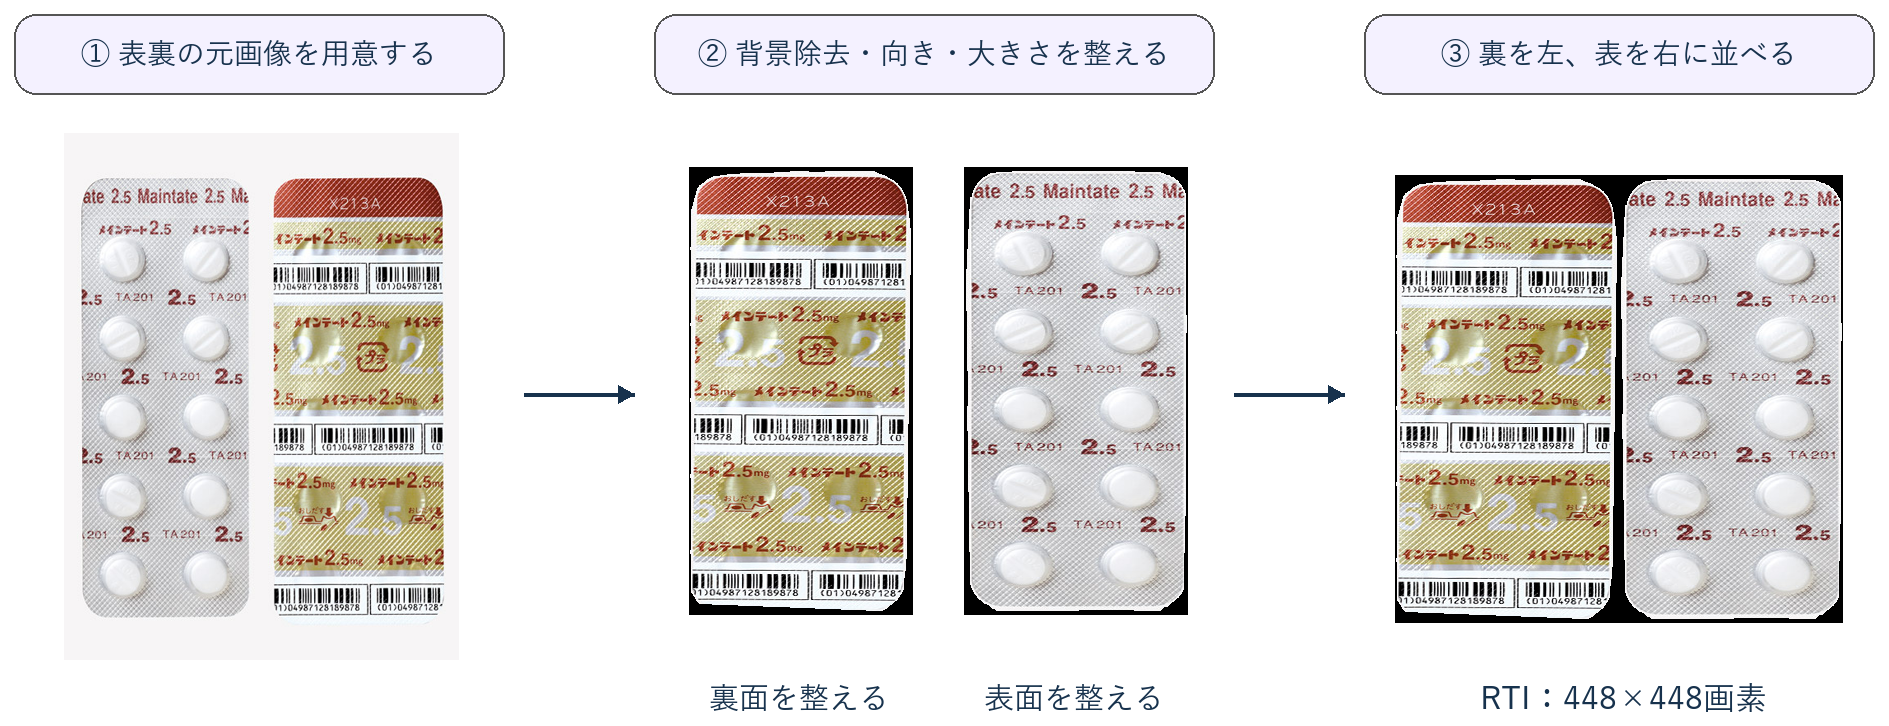
\includegraphics[width=\linewidth]{figures/generated/rti_from_collected.png}
  \caption[収集画像の表面・裏面からRTIを作成する手順]{収集画像の表面・裏面からRTIを作成する手順（メインテート錠2.5mgの例）．単剤の主結果r16\_a128ではRTIそのものは学習しない．田辺ファーマの製剤写真を加工して作成した\cite{tanabe_mnt_photo}．}
  \label{fig:rti}
\end{figure}

各面から，フルシート1枚，1錠区画8枚，縦2分割画像2枚，縦4分割画像4枚を生成する．
1錠区画は，各面の前景外接矩形へ薬剤ごとに定めた固定格子を当て，左上から行優先で最大8枚を切り出したものである．
縦2分割画像と縦4分割画像は，前景外接矩形を高さ方向へ等分した水平帯である．
この切り出しは既知のPTP配列に基づく固定規則であり，任意の包装に対する一般的な錠剤セル検出器ではない．
通常の薬剤で生成する基画像数$N_d$は，RTIを含めて式\eqref{eq:base_count}の31枚となる．
レボフロキサシン錠500mgは，錠剤セル数の制約により1錠区画を各面5枚とし，25枚となる．
41薬剤の基画像は，式\eqref{eq:base_total}の合計1,265枚である．
RTIを除くと1,224枚となる．

\begin{equation}
  N_d = 1 + 2(1 + 8 + 2 + 4) = 31
  \label{eq:base_count}
\end{equation}

\begin{equation}
  N_{\mathrm{base}} = 40 \times 31 + 1 \times 25 = 1{,}265
  \label{eq:base_total}
\end{equation}

図\ref{fig:exp82_training_images}に，RTIを除いた1薬剤分の学習用画像30枚の例を示す．
アルゴリズム\ref{alg:image_generation}に，基画像生成の手順を示す．

\begin{figure}[htbp]
  \centering
  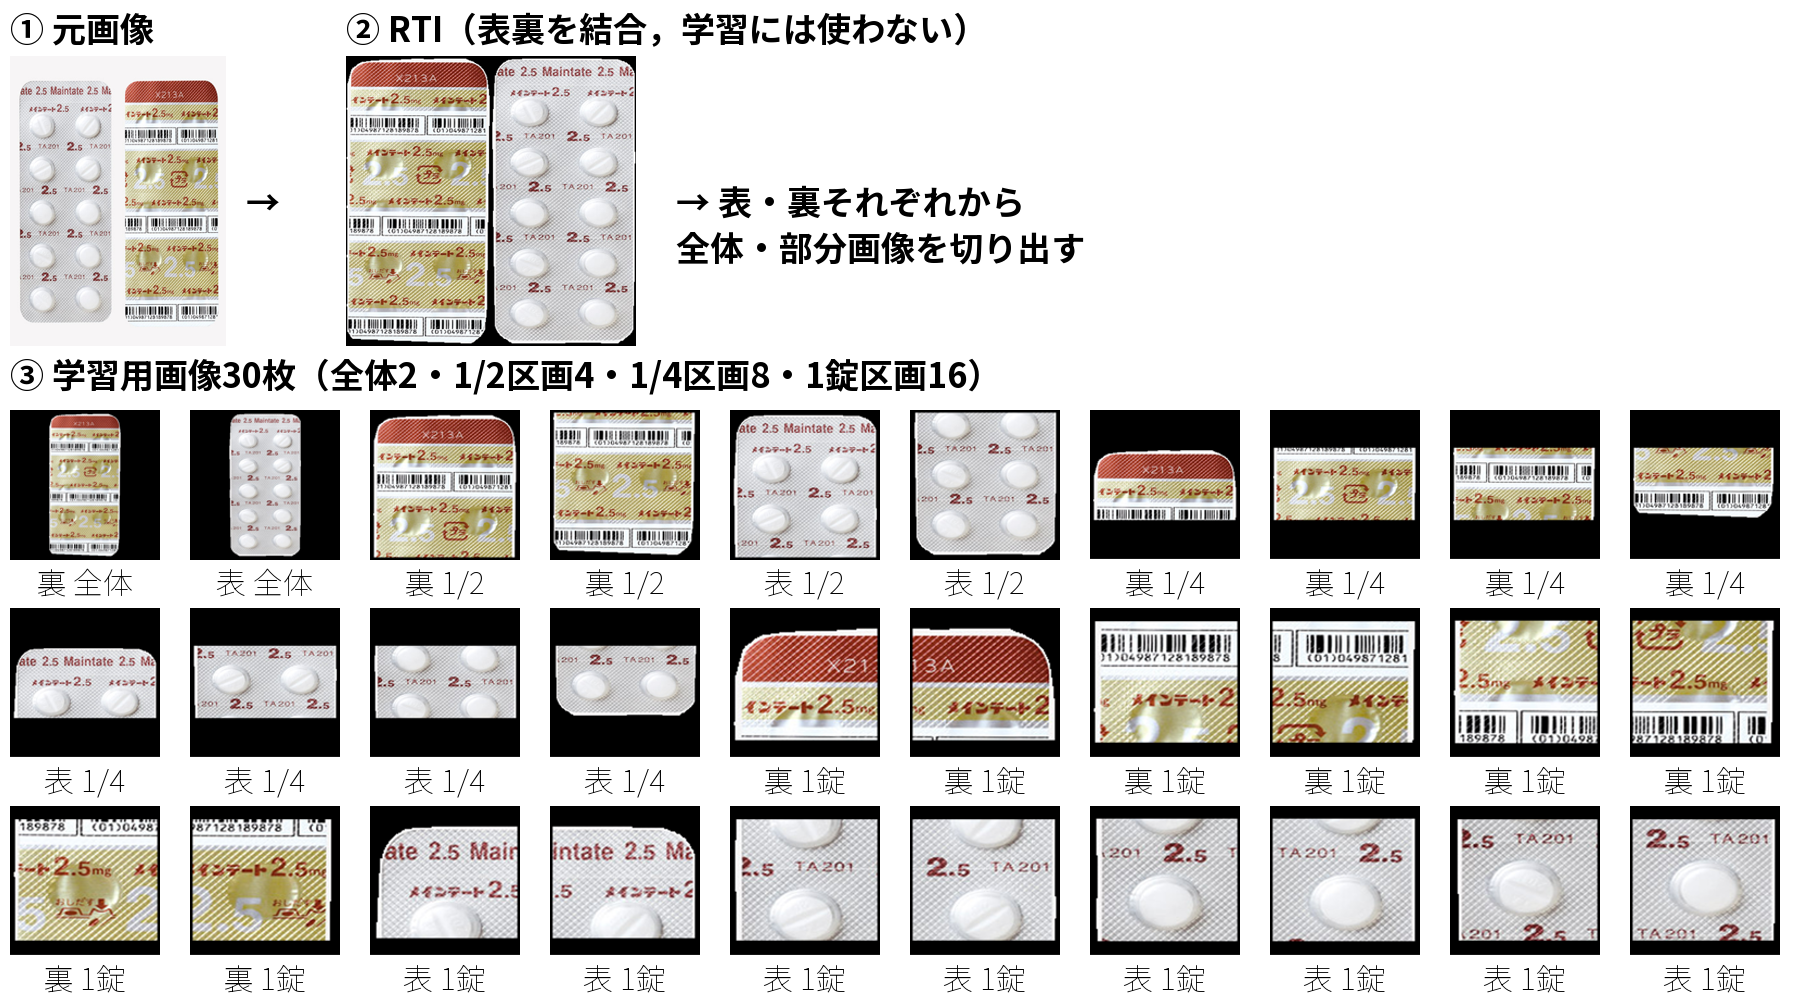
\includegraphics[width=\linewidth]{figures/generated_ver10/exp82_training_images_a.png}
  \caption[元画像・RTI・学習用画像30枚の例]{元画像，RTI，学習用画像30枚の例（メインテート錠2.5mg，全体2枚，1/2区画4枚，1/4区画8枚，1錠区画16枚）．RTI自体は学習から除外した．田辺ファーマの製剤写真を加工して作成した\cite{tanabe_mnt_photo}．}
  \label{fig:exp82_training_images}
\end{figure}

\begin{algorithm}[H]
  \caption{収集画像からの基画像生成}
  \label{alg:image_generation}
    \begin{algorithmic}[1]
    \REQUIRE 薬剤$d$の表面画像$I_{d,f}$，裏面画像$I_{d,b}$
    \ENSURE 基画像集合$\mathcal{D}_d$
    \STATE $\mathcal{D}_d \gets \emptyset$
    \STATE 表裏画像から背景を除去し，PTP包装の凸包を抽出する
    \STATE 透視変換により，表裏画像の向きと大きさを正規化する
    \STATE 裏面を左，表面を右へ配置してRTIを生成する
    \STATE 生成したRTIを$\mathcal{D}_d$へ追加する
    \STATE 正規化した表裏フルシートを$\mathcal{D}_d$へ追加する
    \FOR{面$s \in \{f,b\}$}
      \STATE $T(I_{d,s})$の前景外接矩形へ薬剤$d$に対応する固定格子を設定する
      \STATE 格子区画に対応する部分画像を，左上から行優先で最大8枚生成する
      \STATE 前景外接矩形を高さ方向へ2等分し，水平帯を2枚生成する
      \STATE 前景外接矩形を高さ方向へ4等分し，水平帯を4枚生成する
      \STATE 生成画像を$\mathcal{D}_d$へ追加する
    \ENDFOR
    \STATE 各画像を448 $\times$ 448の黒背景へ配置する
    \RETURN $\mathcal{D}_d$
  \end{algorithmic}
\end{algorithm}

\subsection{画像拡張}

本報告書では，2種類の画像拡張セット（各17種）を用いる．
単剤の主結果r16\_a128は，回転12条件と明度5条件からなる\texttt{v3\_17}を用いる．
回転は0度から330度まで30度刻みとし，明度倍率は0.8，0.9，1.0，1.1，1.2とする．
回転と明度変化は別々に適用するため，拡張数は式\eqref{eq:augmentation}の17となる．
0度回転と明度倍率1.0は画素値が同一だが，別レコードとして1回ずつ提示する．

\begin{equation}
  \mathcal{A}_{v3}
  =
  \left(
    R_{0},R_{30},\ldots,R_{330},
    B_{0.8},B_{0.9},B_{1.0},B_{1.1},B_{1.2}
  \right)
  \label{eq:augmentation}
\end{equation}

従来の主結果であるver4条件Dは，撮影時の変動を模擬する別の17種（\texttt{acquisition\_17}）を用いる．
内訳は，無変換1条件，回転6条件，明度2条件，コントラスト2条件，ガンマ2条件，台形歪み2条件，ぼかし1条件，ノイズ1条件である．
ver4条件Dでは，1エポック当たりの総提示数が1,265$\times$17$=$21,505枚，5エポックで107,525枚となる．

\subsection{LoRA学習}

基盤モデルには，\ref{sec:vlm}節のQwen3.5-4Bを用いる．
画像サイズは448$\times$448画素とし，プロンプトと正解薬剤名を学習ペアとする．
モデル重みはBF16で読み込み，LoRAのドロップアウト率は0.05とする．
ただしver1からver4条件Aでは，モデルを4ビットに量子化して学習するQLoRAを用いる\footnote{ver1はRTIと1錠区画を基画像とした最初の版，ver4条件Aはver3の設定を基準に学習を再構成した条件である．}．
LoRAの対象は，\texttt{q\_proj}，\texttt{k\_proj}，\texttt{v\_proj}，\texttt{o\_proj}，\texttt{gate\_proj}，\texttt{up\_proj}，\texttt{down\_proj}である．
学習率は$2.0 \times 10^{-4}$，実効バッチサイズは128とし，最適化にはAdamWを用いる．
損失は，プロンプトをマスクし，回答文字列と終端トークンの部分だけで計算する．
推論では貪欲法を用い，最大生成長を32トークンとする．

単剤の主結果r16\_a128は，ランク16，スケーリング係数128，\texttt{v3\_17}を用い，乱数シード42，43，44の3回学習する．
総提示数は107,525枚に固定する．
従来の主結果であるver4条件Dは，ランク16，スケーリング係数32，\texttt{acquisition\_17}，5エポック，乱数シード42の1回学習である．
両者は，RTIの有無，画像拡張セットおよびスケーリング係数が異なる別系統の学習結果である．

\subsection{評価方法}

\subsubsection{単剤評価}\label{sec:single_eval}

単剤評価には，内部開発評価画像287枚を用いる．
内訳は表面212枚，裏面75枚であり，フルシート29枚と，錠剤が1錠から9錠まで残った部分シート258枚を含む．
1クラス当たりの枚数は3枚から10枚であり，クラス間で偏りがある．
学習元の収集画像とは出典と撮影条件が異なる．
図\ref{fig:internal_eval_examples}に，撮影元画像と，背景除去・向き補正・448画素正方形化後のモデル入力の対応例を示す．
各列の上段が撮影元画像，下段がモデル入力である．
撮影元画像内の包装の占有率や向きが異なっても，モデル入力では包装が黒背景の正方形へ正規化される．

\begin{figure}[htbp]
  \centering
  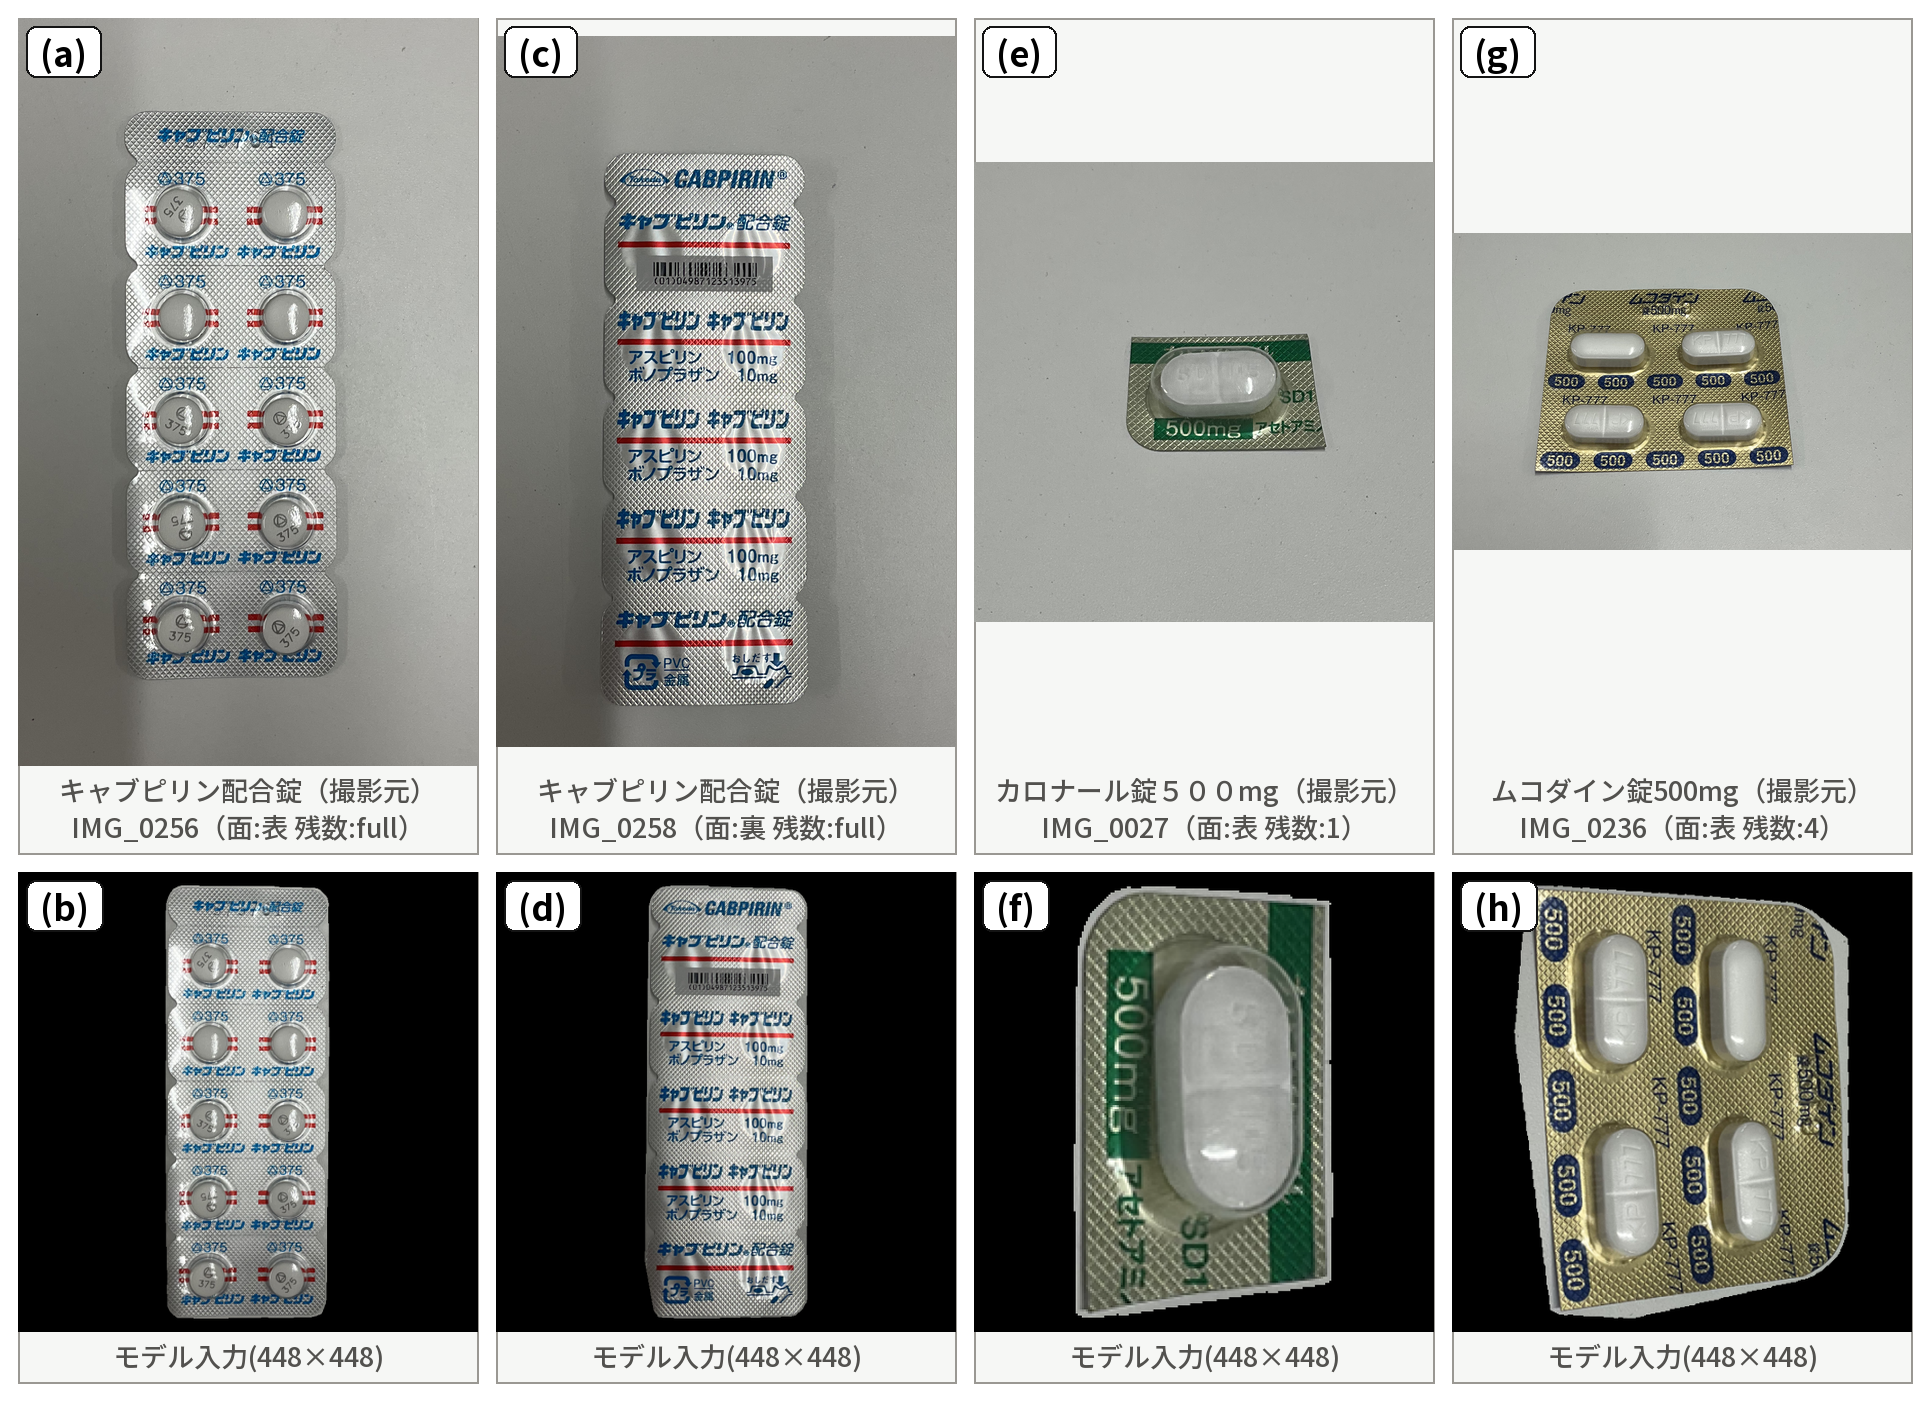
\includegraphics[width=\linewidth]{figures/generated/internal_eval_examples.png}
  \caption[内部開発評価画像の撮影元画像とモデル入力]{内部開発評価画像の撮影元画像（上段）とモデル入力（下段）の対応例．（a）（b）は表面フルシート，（c）（d）は裏面フルシート，（e）（f）は表面1錠，（g）（h）は表面4錠である．大学病院薬剤部で撮影した画像を，著者が保存済みデータから再配置した．}
  \label{fig:internal_eval_examples}
\end{figure}

文字列$s$にNFKC正規化と小文字化を適用し，空白と記号を除去した結果を$g(s)$とする．
一致判定$M(a,b)$は，$g(a)=g(b)$，または$g(a)$が$g(b)$の部分文字列である場合に真とする．
画像$x_i$に対してモデルが生成した回答を$\hat{y}_i$，正解ラベルを$y_i$として，正解率は式\eqref{eq:top1}で求める．

\begin{equation}
  \operatorname{Accuracy}
  =
  \frac{1}{n}
  \sum_{i=1}^{n}
  \mathbf{1}\!\left(M(y_i,\hat{y}_i)\right)
  \label{eq:top1}
\end{equation}

ここで，$n=287$は評価画像数，$\mathbf{1}$は判定が真なら1，偽なら0となる関数である．百分率では式\eqref{eq:top1}の値を100倍する．
この判定は，正規化後の完全一致より緩い．
そのため，保存済みの予測を完全一致でも集計し，正解数の違いを確認する．
結果は\ref{sec:env_data}節に示す．

同じ画像に対する2つの条件の正誤を比較する場合は，対応のある二値データとしてMcNemar検定を用いる．
一方の条件だけが正解した画像の枚数を使い，両側の正確検定で比較する．
学習を3回行った条件では，各回の結果をそれぞれ比較する．
比較が1つの場合は，$p<0.05$を有意の基準とする．複数の比較では，偶然の差を有意と判断しやすくなるため，比較数に応じて基準を厳しくする．
% 保存済みの検定はBonferroni補正を使用。14比較、3比較、6比較の設定と数値は変更しない。
有意差が認められない結果は，2条件が同等であることを示すものではない．
また，287枚には同じクラスの複数画像が含まれ，画像対の独立性は確認できない．
そのため，検定結果は今回の287枚についての比較として扱い，他の薬剤や撮影条件でも同じ差が出るとは判断しない．

学習元は薬剤ごとに1組の収集画像であり，評価対象は内部開発評価画像である．
このため，5分割交差検証は用いず，全287枚の正解率を主な集計値とする．

\subsubsection{比較実験}

追加学習前の基準として，LoRAを適用していないQwen3.5-4Bを，ver4条件Dと同じ287枚，入力形式，プロンプト，生成条件で評価する．
プロンプトに候補一覧は含めず，採点は正解薬剤名が出力に含まれていれば正解とする包含採点とする．
比較対象はver4条件Dであり，単剤の主結果r16\_a128とLoRAなしの直接比較は行っていない．

外部サービスとの比較には，Gemini 3.8 Flashの短文条件，Gemini 3.8 Flashの候補一覧付き条件，およびGemini 3.5 Flashの短文条件を用いる．
短文条件では，Qwenと同じ画像と同じプロンプトを入力し，候補を与えない．
候補一覧付き条件では，41薬剤の一覧から1つを選ばせる．
Qwenの評価と同じ前処理済み448$\times$448画素の画像を入力する．
温度0，最大出力トークン4096で，287枚を各1回評価した保存予測を用いる．
採点は，r16\_a128と同じ包含採点とする．

\subsubsection{信頼ゲート}

信頼ゲートは，モデルが生成した薬剤名を，次の3段階で確認し，1つでも満たさなければ回答を保留する．
第1段階では，出力が学習した41薬剤の名前と一致することを確認する．
第2段階では，回転，反転，明度などを加えた11視点のテスト時拡張を行う．
多数決の結果がTop-1と一致し，一致率がしきい値以上であることを確認する．
第3段階では，Top-3ビーム探索の第1候補の系列スコアと，第1候補と第2候補の差がしきい値以上であることを確認する．
図\ref{fig:trust_gate_pipeline}に，判定の順序を示す．

\begin{figure}[htbp]
  \centering
  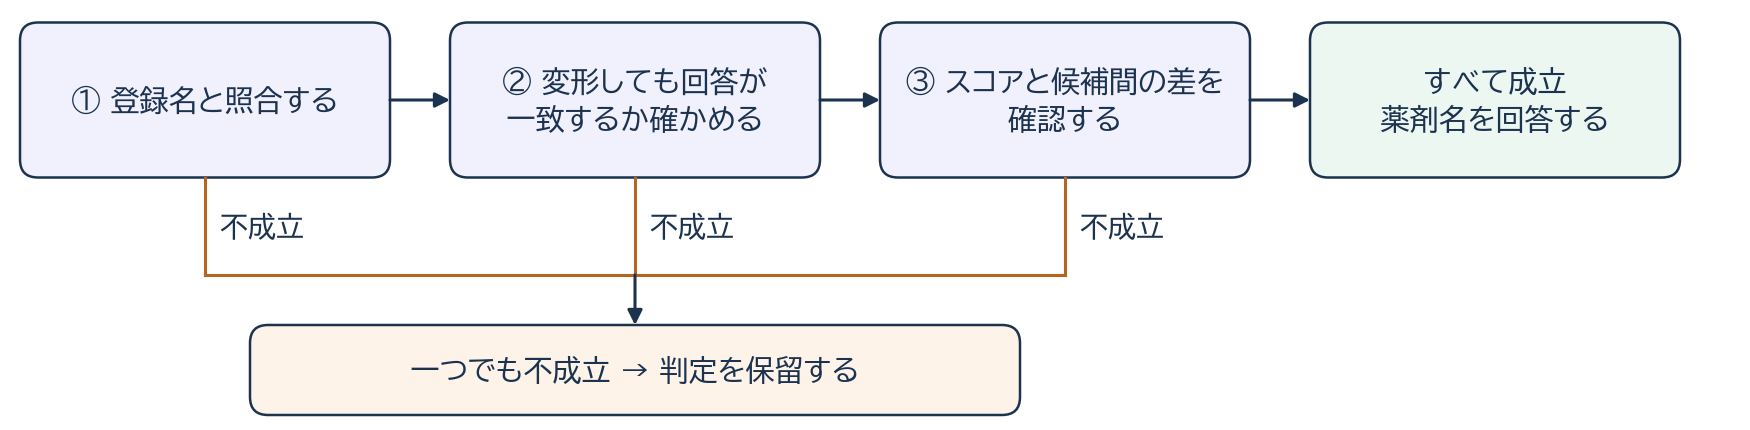
\includegraphics[width=\linewidth]{figures/generated_ver10/trust_gate_pipeline.png}
  \caption[信頼ゲートによる回答と保留の判定手順]{信頼ゲートによる回答と保留の判定手順．登録名と照合する第1段階，変形しても回答が一致するか確かめる第2段階，スコアと候補間の差を確認する第3段階の順に判定し，1つでも不成立であれば判定を保留する．しきい値はモデルごとに校正集合で決める．}
  \label{fig:trust_gate_pipeline}
\end{figure}

既知薬剤には内部開発評価画像287枚を用い，記録ラベル単位で校正集合139枚と最終評価集合148枚に事前分割する．
未知薬剤には，学習した41薬剤に含まれない薬剤の収集画像125枚を用い，薬剤ラベル単位で校正集合67枚と最終評価集合58枚に事前分割する．
未知薬剤に対して既知薬剤名を回答することを，危険通過と呼ぶ．
しきい値は校正集合だけで決め，最終評価集合の推論前に固定する．
決め方は，既知薬剤の誤回答を0件，未知薬剤の危険通過を67枚中3枚以下とする制約下で，既知薬剤への正しい回答数を最大にすることである．
信頼ゲートは，ver4条件D（ランク16・係数32）とver6（ランク32・係数64）へ適用し，主結果r16\_a128への適用は扱わない．

\subsubsection{隙間のない合成複数薬剤画像}

薬剤数が未知の複数薬剤入力に対する探索的評価として，隙間のない元写真タイル（固定800枚）を用いる．
元写真を768$\times$1024画素へ縦横比を保ってリサイズし，タイル間隔と外周余白を0画素として連結する．
薬剤数は2，3，5，8の4条件，各200枚，計800枚である．
検出器には薬剤数，配置および薬剤名を入力しない．
Cannyエッジ検出と輪郭抽出で候補領域を作り，前景強度の高い順に最大10領域を残す．
各領域を黒背景448$\times$448画素へ整形して単剤モデルへ入力する．

最大10候補が正解薬剤をすべて含めば，余分な予測を許して画像を成功とする方式をTop-10方式と呼ぶ．
Top-10方式は過検出を罰しない．
同じ推論結果から，正解薬剤数$N$を既知として候補1位から$N$位だけを残し，正解薬剤と1対1で完全一致した画像を成功とする方式をTop-N方式と呼ぶ．
Top-N方式は，評価時点でのみ既知となる$N$を用いるため，薬剤数が未知の実運用での性能を示すものではない．
本評価は，タイル合成画像によるものであり，薬剤が自由な位置や向き，重なりで置かれる実環境の性能を示すものではない．


%----------------------------------------------------------------------
\clearpage
\section{実験結果・考察}\label{sec:results}
%----------------------------------------------------------------------

\subsection{実験環境と評価データ}\label{sec:env_data}

実験環境を表\ref{tab:environment}に示す．
表\ref{tab:environment}の2条件の学習には，NVIDIA H100を1台ずつ使用した．
固定800枚に対するr16\_a128の評価は，NVIDIA GeForce RTX 4070 Ti SUPER（VRAM 15.992 GiB）で推論のみを行った．
モデルリビジョンと乱数シードを固定した．
ただし，速度を優先してCUDAの決定論的アルゴリズムを無効にした．
このため，ビット単位で同一の再現は保証されない．
本研究は人を対象とする実験ではなく，被験者は用いなかった．
評価画像はPTP包装だけを写した画像であり，患者を識別できる情報は含まれなかった．

\begin{table}[htbp]
  \centering
  \caption{学習の実験環境と設定}
  \label{tab:environment}
  \small
  \setlength{\tabcolsep}{3pt}
  \begin{tabular}{|>{\raggedright\arraybackslash}p{3.0cm}|>{\raggedright\arraybackslash}p{4.7cm}|>{\raggedright\arraybackslash}p{4.7cm}|}
    \hline
    項目 & ver4条件D & r16\_a128 \\ \hline
    GPU & NVIDIA H100，VRAM 93.096 GiB，1台 & 同左 \\ \hline
    OS／Python & Linux 6.8.0，glibc 2.39／Python 3.13.5 & Linux 6.8.0，glibc 2.39／Python 3.12.3 \\ \hline
    主要ライブラリ & PyTorch 2.11.0，CUDA 12.8，cuDNN 9.19，Transformers 5.14.1，PEFT 0.19.1 & PyTorch 2.11.0+cu128，Transformers 5.14.1，PEFT 0.19.1 \\ \hline
    基盤モデル & \multicolumn{2}{p{9.7cm}|}{\shortstack[l]{Qwen/Qwen3.5-4B，リビジョン\\\texttt{851bf6e806efd8d0a36b}\\\texttt{00ddf55e13ccb7b8cd0a}}} \\ \hline
    LoRA & ランク16，係数32，BF16 & ランク16，係数128，BF16 \\ \hline
    画像拡張 & \texttt{acquisition\_17} & \texttt{v3\_17} \\ \hline
    基画像数／総提示数 & 1,265枚／107,525枚 & 1,224枚／107,525枚 \\ \hline
    バッチ & マイクロバッチ16，勾配累積8，実効128 & 実効128 \\ \hline
    乱数シード & 42 & 42，43，44 \\ \hline
  \end{tabular}
\end{table}

内部開発評価画像は41薬剤・287枚であり，1薬剤当たり3〜10枚（平均7枚）であった．
撮影場所は近畿大学病院薬剤部であり，撮影元画像はすべて3,024$\times$4,032画素のPNG形式であった．
撮影元画像のディレクトリ名は2026年4月9日撮影を示した．
一方，撮影端末，距離，角度，照明および背景は保存記録から確認できなかったため，推測で補わなかった．

収集元の保存ファイルは41薬剤・42ファイルであり，表裏が1ファイルに含まれる場合があった．表裏を分けた学習元は各薬剤2枚，計82枚であった．
収集画像は，現行または削除前の収集記録と照合して出典を確認した．
32ファイルは現行の収集記録と直接照合でき，残る10ファイルは削除前の収集記録から出典候補を確認した．
この10ファイルは，収集時の元ファイルから現存する収集画像までの加工履歴をたどれなかった．
また，収集画像と内部開発評価画像287枚に同一の画像は含まれていなかった．

評価の判定規則について，保存済み予測を正規化後の完全一致で再集計した．
その結果，単剤の正解数は，ver4条件D，ver4条件C，ver6，ver7で，287枚中それぞれ280枚，283枚，286枚，284枚であった．
これらは，包含判定の集計値と変わらなかった\footnote{ver4条件CはBF16 LoRAでランク16・係数32，全射影層を学習対象とした条件である．ver7はver6を基に基画像を1,347枚へ増やし，41候補から選ぶ推論へ変えた条件である．}．

\subsection{初期実画像方式と収集画像学習への移行}

研究初期には，撮影した287枚を撮影画像単位で213枚の学習用と74枚の評価用に分け，Qwen3.5-4BをLoRAで追加学習した．
評価用の74枚では74枚すべてで正解した．
同じ287枚を5分割する交差検証では，全分割を統合して283/287（98.6\%）であった．
1薬剤当たりの学習元画像数を変えた比較では，6枚以上の撮影画像を持つ33薬剤の固定評価79枚に対し，1枚で67.1\%，2枚で87.3\%，4枚で91.1\%，利用可能な全画像（5〜8枚）で98.7\%であった．
ただし，いずれも乱数シード42の1回の比較であり，必要撮影枚数を確定する結果ではなかった．
薬剤を追加するたびに複数の学習用実画像を撮影する負担が，対象薬剤数を増やすうえでの課題となった．
そこで，フルシート表裏の収集画像を学習元とする方式へ移行した．

\subsection{収集画像学習ver1からver9}\label{sec:ver1_v9}

収集画像学習では，いずれも同じ内部開発評価画像287枚を評価し，基画像の構成と学習設定を段階的に変更した．
図\ref{fig:ver_lineage}に，各版の関係と単剤正解率を示す．
乱数シード42の1回の学習による値であった．
内部開発評価画像は学習に用いなかったが，条件検討に繰り返し使用した．

\begin{figure}[htbp]
  \centering
  \begin{tikzpicture}[
    ver/.style={draw, rectangle, rounded corners=2pt, minimum width=3.0cm, minimum height=1.35cm, align=center, font=\footnotesize, inner sep=2pt},
    mainv/.style={ver, fill=blue!15, line width=0.8pt},
    arr/.style={-{Stealth[length=2mm]}, thick},
    lab/.style={font=\scriptsize, align=center, text width=2.4cm, inner sep=1pt},
    vlab/.style={font=\scriptsize, align=left, text width=2.0cm, inner sep=1pt, anchor=west}]
    \node[ver] (v1) at (0,0) {\textbf{ver1}\\259/287（90.24\%）\\基画像457枚};
    \node[ver] (v2) at (5.6,0) {\textbf{ver2}\\255/287（88.85\%）\\基画像451枚};
    \node[ver] (v3) at (11.2,0) {\textbf{ver3}\\281/287（97.91\%）\\基画像1,265枚};
    \node[ver] (a) at (0,-2.9) {\textbf{ver4条件A}\\272/287（94.77\%）\\基画像1,265枚};
    \node[ver] (b) at (5.6,-2.9) {\textbf{ver4条件B}\\276/287（96.17\%）\\基画像1,265枚};
    \node[ver] (c) at (11.2,-2.9) {\textbf{ver4条件C}\\283/287（98.61\%）\\基画像1,265枚};
    \node[ver] (v7) at (0,-5.8) {\textbf{ver7}\\284/287（98.95\%）\\基画像1,347枚};
    \node[ver] (v6) at (5.6,-5.8) {\textbf{ver6}\\286/287（99.65\%）\\基画像1,265枚};
    \node[mainv] (d) at (11.2,-5.8) {\textbf{ver4条件D}\\280/287（97.56\%）\\基画像1,265枚};
    \node[ver] (v8) at (0,-8.7) {\textbf{ver8}$^{\ast}$\\286/287（99.65\%）\\基画像1,347枚};
    \node[ver] (v9) at (5.6,-8.7) {\textbf{ver9}$^{\ast}$\\286/287（99.65\%）\\基画像1,347枚};
    \node[ver] (v5) at (11.2,-8.7) {\textbf{ver5-2・5-3}\\281/287（97.91\%）\\基画像1,347枚};
    \draw[arr] (v1) -- node[lab, above] {表裏を分離し，面別の部分画像を追加} (v2);
    \draw[arr] (v2) -- node[lab, above] {異なる錠剤セル，縦2・4分割を追加} (v3);
    \draw[arr] (v3.south) -- (11.2,-1.7) -- (0,-1.7) -- (a.north);
    \node[lab, text width=5.5cm] at (5.6,-1.7) [above] {ver3を基準に4ビットQLoRAを再構成};
    \draw[arr] (a) -- node[lab, above] {BF16 LoRAへ変更} (b);
    \draw[arr] (b) -- node[lab, above] {ランク16・係数32，全射影層を対象に拡大} (c);
    \draw[arr] (c.south) -- (d.north) node[vlab, midway, xshift=2mm] {拡張を重複のない17種へ変更};
    \draw[arr] ([xshift=-1.0cm]c.south) -- ([xshift=-1.0cm]c.south |- 0,-4.35) -- (5.6,-4.35) -- (v6.north);
    \node[lab, text width=3.4cm] at (7.9,-4.35) [below] {ランク32・係数64へ増加（探索的追試）};
    \draw[arr] (v6) -- node[lab, above] {基画像を1,347枚にし，41候補から選ぶ推論へ変更} (v7);
    \draw[arr] (v7) -- (v8) node[vlab, midway, xshift=2mm] {総提示数をver6と同数に固定};
    \draw[arr] (v8) -- node[lab, above] {明度1.0の拡張を解像度劣化に置換} (v9);
    \draw[arr] (d) -- (v5) node[vlab, midway, xshift=2mm] {表面中央の縦2・4分割を追加};
  \end{tikzpicture}
  \caption{収集画像学習ver1からver9の関係（箱は上から版名，単剤正解数，基画像数を，矢印は基にした版と変更点を表す．評価は同じ内部開発評価画像287枚，各1回学習である．色付きの箱は従来の主結果ver4条件Dであり，＊は各アダプタ自身を単剤評価した診断値である）}
  \label{fig:ver_lineage}
\end{figure}

図\ref{fig:ver_lineage}のとおり，ver1からver4条件Cまでは，基画像の構成と学習設定を1段階ずつ変更した．
ver4条件Cからは，画像拡張を変えたver4条件Dと，LoRAの容量を増やしたver6の2つへ分かれた．
ver5は，ver4条件Dを再実行した条件（ver5-1），表面中央の縦2分割・縦4分割画像を加えた条件（ver5-2），ver5-2の総提示数をver5-1と同数にそろえた条件（ver5-3）の3条件であった．
ver7からver9は，ver6を基に，基画像を1,347枚へ増やした条件であった．

ver1は90.24\%であった．
ver2では，同じ位置の1錠区画を重複して用いており，88.85\%へ低下した．
ver3では，異なる錠剤セル，縦2分割画像および縦4分割画像を加えて基画像を1,265枚とした．
その結果，97.91\%へ上昇した．
ただし，ver2からver3では基画像の構成，画像枚数，使用GPUおよび実効バッチが同時に変化した．
したがって，改善を部分画像の追加だけに分けて説明できなかった．

ver4条件AからDは，量子化，LoRAのランクと係数，学習対象層，画像拡張を変更した比較であった．
条件Aはver3と同じ設定を意図したが，94.77\%であった．
ver3の結果は再現されなかった．
条件Cは98.61\%と最も高く，条件Dは97.56\%であった．
各比較では複数の要因を同時に変更したため，BF16化や学習対象層の拡大だけの効果とは解釈できなかった．
ver4条件Dは，実験の開始前に主結果として定めた設定であり，本報告書では従来の主結果（別系統）として扱った．
ただし，第三者が検証できる形で事前に登録した条件ではなかった．

ver4条件Dの保存済み予測を，面，シート種別および残存錠数で層別に再集計した結果を表\ref{tab:condition_d_stratified}に示す．
裏面75枚とフルシート29枚は，誤分類が0件であった．
一方，誤分類7件はすべて表面に生じた．
ただし，残存錠数別の分母は3枚から60枚までばらついており，錠数と正解率の関係を確定的には解釈できなかった．

\begin{table}[htbp]
  \centering
  \caption{ver4条件Dの層別正解率（分母は内部開発評価画像287枚の内訳）}
  \label{tab:condition_d_stratified}
  \small
  \begin{tabular}{|l|l|r|r|}
    \hline
    層 & 区分 & 正解数／枚数 & 正解率 \\ \hline
    \multirow{2}{*}{面} & 表 & 205/212 & 96.70\% \\ \cline{2-4}
     & 裏 & 75/75 & 100.00\% \\ \hline
    \multirow{2}{*}{シート種別} & フルシート & 29/29 & 100.00\% \\ \cline{2-4}
     & 部分シート & 251/258 & 97.29\% \\ \hline
    \multirow{9}{*}{残存錠数} & 1錠 & 37/39 & 94.87\% \\ \cline{2-4}
     & 2錠 & 60/60 & 100.00\% \\ \cline{2-4}
     & 3錠 & 40/42 & 95.24\% \\ \cline{2-4}
     & 4錠 & 42/44 & 95.45\% \\ \cline{2-4}
     & 5錠 & 33/33 & 100.00\% \\ \cline{2-4}
     & 6錠 & 15/16 & 93.75\% \\ \cline{2-4}
     & 7錠 & 15/15 & 100.00\% \\ \cline{2-4}
     & 8錠 & 6/6 & 100.00\% \\ \cline{2-4}
     & 9錠 & 3/3 & 100.00\% \\ \hline
    全体 & 全画像 & 280/287 & 97.56\% \\ \hline
  \end{tabular}
\end{table}

表\ref{tab:condition_d_errors}に誤分類7件の内訳を示す．
正解側ではムコダイン錠500mgが2件，ほか5薬剤が各1件であった．
予測先ではデエビゴ錠5mgが3件，ほか4薬剤が各1件であり，41薬剤外の文字列はなかった．
図\ref{fig:condition_d_errors}に，代表的な4件のモデル入力を示す．
誤分類数が少なく，包装の向き，錠数または印字が原因であるとは断定できなかった．

\begin{table}[htbp]
  \centering
  \caption{ver4条件Dの誤分類7件（内部開発評価画像287枚）}
  \label{tab:condition_d_errors}
  \small
  \setlength{\tabcolsep}{3pt}
  \begin{tabular}{|p{1.7cm}|p{3.6cm}|p{4.2cm}|c|c|}
    \hline
    画像ID & 正解薬剤 & ver4条件Dの予測 & 面 & 錠数 \\ \hline
    IMG\_0020 & レバミピド錠100mg & プレドニン錠5mg & 表 & 1 \\ \hline
    IMG\_0027 & カロナール錠500mg & デエビゴ錠5mg & 表 & 1 \\ \hline
    IMG\_0039 & ミヤBM錠 & メチコバール錠500$\mu$g & 表 & 3 \\ \hline
    IMG\_0047 & タケキャブ錠20mg & ジャディアンス錠10mg & 表 & 3 \\ \hline
    IMG\_0079 & メトクロプラミド錠5mg & デエビゴ錠5mg & 表 & 4 \\ \hline
    IMG\_0236 & ムコダイン錠500mg & レボチロキシンNa錠50$\mu$g & 表 & 4 \\ \hline
    IMG\_0238 & ムコダイン錠500mg & デエビゴ錠5mg & 表 & 6 \\ \hline
  \end{tabular}
\end{table}

\begin{figure}[htbp]
  \centering
  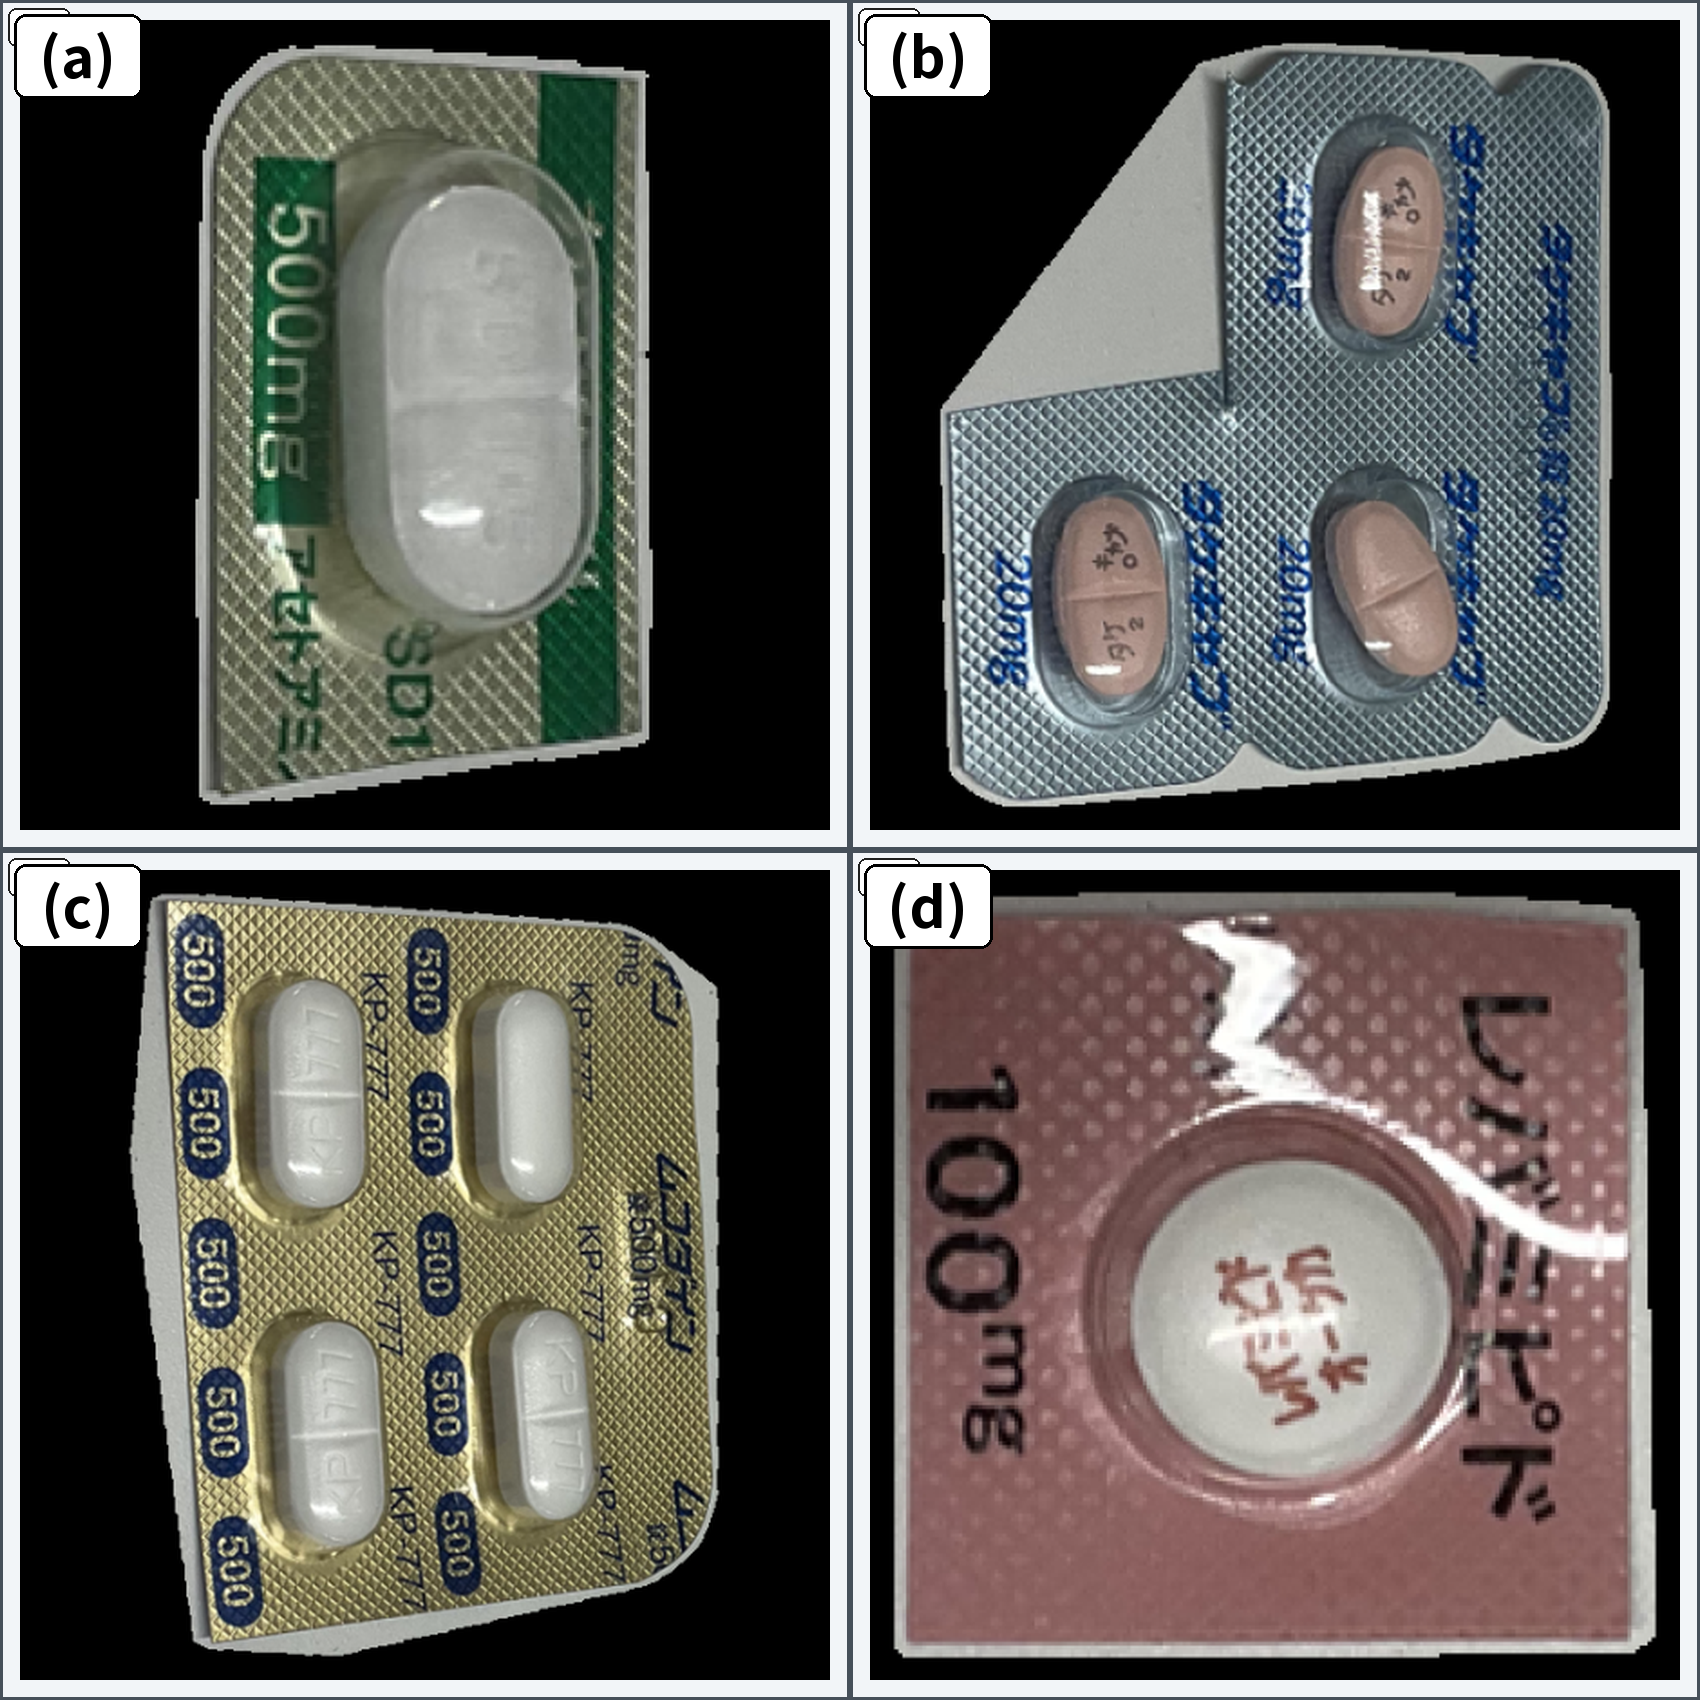
\includegraphics[width=0.78\linewidth]{figures/generated_ver10/condition_d_errors_2x2.png}
  \caption[ver4条件Dの代表的な誤分類モデル入力]{ver4条件Dの代表的な誤分類モデル入力．
  （a）IMG\_0027：カロナール錠500mg$\rightarrow$デエビゴ錠5mg，
  （b）IMG\_0047：タケキャブ錠20mg$\rightarrow$ジャディアンス錠10mg，
  （c）IMG\_0236：ムコダイン錠500mg$\rightarrow$レボチロキシンNa錠50$\mu$g，
  （d）IMG\_0020：レバミピド錠100mg$\rightarrow$プレドニン錠5mgである．
  著者が保存済みモデル入力を再配置した．}
  \label{fig:condition_d_errors}
\end{figure}


ver5では，表面中央の縦2分割画像と縦4分割画像を追加しても，281/287であった．
追加前の280/287に対する正確McNemar検定は$p=1.00$であった．
ver6は，ver4条件Cからランクを16から32へ，係数を32から64へ増やした．
正解は，ver4条件Cのみが1枚，ver6のみが4枚であり，正確McNemar検定は$p=0.375$で有意差はなかった．
ver6の誤分類1件（IMG\_0236）は，ver4条件Cが正解していた画像であり，改善の向きは一様ではなかった．
ver7，ver8およびver9も286/287以下であり，ver6を上回らなかった．
ver8・ver9は，ver6と同じ286/287であるが，誤分類した画像は条件ごとに異なった．
ver6，ver8およびver9は，結果を確認した後に選んだ条件であり，探索的な最高観測値として扱った．
いずれも乱数シード42の1回の学習であり，286/287という同数の観測から，条件間の優劣と再現性は判断できなかった．

ver1からver9で正解率が上がった理由には，部分画像の追加，LoRAのランクの増加，学習枚数の差が関係したと考えた．
ただし，これらは同時に変わっており，それぞれの効果は分けて確かめなかった．

\subsection{追加学習していないQwen3.5-4Bとの比較}\label{sec:qwen_baseline}

LoRAを適用していないQwen3.5-4Bを，ver4条件Dと同じ287枚，入力形式，プロンプト，生成条件で評価した．
結果を表\ref{tab:qwen_baseline}に示す．
LoRAなしは3/287（1.05\%），ver4条件Dは280/287（97.56\%）であった．
正規化後の出力が正解薬剤名と完全一致した画像は，LoRAなしが0/287であり，ver4条件Dは280/287であった．
同じ画像で比べると，LoRAなしだけが正解した画像は0枚，ver4条件Dだけが正解した画像は277枚であった．
正確McNemar検定（両側）の$p$値は$8.24\times10^{-84}$であった．
この比較は1つであり，有意水準は0.05とした．

\begin{table}[htbp]
  \centering
  \caption{追加学習していないQwen3.5-4Bとver4条件Dの比較（内部開発評価画像287枚，候補一覧なし，包含採点，各1回）}
  \label{tab:qwen_baseline}
  \small
  \begin{tabular}{|p{5.2cm}|r|r|r|}
    \hline
    モデル & 正解数 & 正解率 & 完全一致 \\ \hline
    追加学習していないQwen3.5-4B & 3/287 & 1.05\% & 0/287 \\ \hline
    ver4条件D（LoRAあり） & 280/287 & 97.56\% & 280/287 \\ \hline
  \end{tabular}
\end{table}

LoRAなしで正解となった3枚も，出力文の中に正解薬剤名が含まれていたものであり，薬剤名だけを答えた出力は0枚であった．
今回の条件では，LoRAで追加学習したモデルの正解率が高かった．
LoRAによる追加学習で，対象薬剤の特徴を学べたためと考えた．
ただし，比較対象はver4条件Dであり，単剤の主結果r16\_a128とLoRAなしの直接比較は行わなかった．
また，LoRAなしの出力形式も異なったため，正解数だけでは誤りの原因を判断できなかった．
LoRAなしは1回の評価，ver4条件Dは乱数シード42の1回学習であり，287枚は内部開発評価画像であった．
このため，新しく撮影した画像で97.56\%を再現した証拠ではない．

\subsection{主結果r16\_a128の選定と追加検証}\label{sec:r16a128_addendum}

\subsubsection{LoRA容量の系統比較と主結果の選定}\label{sec:r16a128_sweep}

ver6は，ランク32・係数64・乱数シード42の1回の観測であった．
複数の設定と複数回の学習による系統的な比較は行っていなかった．
そこで，画像拡張セットを\texttt{v3\_17}に固定し，LoRAのランク8から64，係数8から128の8条件を設定した．
基画像は1,224枚，総提示数は107,525枚，学習率は0.0002，実効バッチは128，計算精度はBF16とした．
各条件を乱数シード42，43，44の3回ずつ比較した．6条件は新たに学習し，残る2条件は設定が一致する既存の結果を用いた．
結果を表\ref{tab:r16a128_sweep}に示す．

\begin{table}[htbp]
  \centering
  \caption{v3\_17拡張・LoRAランクとスケーリング係数の系統比較（内部開発評価画像287枚の単剤正解率，3回の学習）}
  \label{tab:r16a128_sweep}
  \small
  \setlength{\tabcolsep}{3pt}
  \begin{tabular}{|l|c|c|r|r|r|r|}
    \hline
    条件 & ランク & 係数 & seed42 & seed43 & seed44 & 平均$\pm$標本SD \\ \hline
    r08\_a16 & 8 & 16 & 98.61\% & 97.91\% & 98.26\% & 98.26\%$\pm$0.35pt \\ \hline
    r16\_a08 & 16 & 8 & 98.61\% & 97.91\% & 98.26\% & 98.26\%$\pm$0.35pt \\ \hline
    r16\_a16 & 16 & 16 & 98.95\% & 97.91\% & 99.30\% & 98.72\%$\pm$0.73pt \\ \hline
    r16\_a32 & 16 & 32 & 99.65\% & 98.95\% & 98.26\% & 98.95\%$\pm$0.70pt \\ \hline
    r16\_a64 & 16 & 64 & 97.91\% & 98.26\% & 98.61\% & 98.26\%$\pm$0.35pt \\ \hline
    \textbf{r16\_a128} & \textbf{16} & \textbf{128} & \textbf{99.65\%} & \textbf{100.00\%} & \textbf{98.95\%} & \textbf{99.54\%$\pm$0.53pt} \\ \hline
    r32\_a64 & 32 & 64 & 99.65\% & 98.95\% & 97.91\% & 98.84\%$\pm$0.88pt \\ \hline
    r64\_a128 & 64 & 128 & 97.56\% & 99.30\% & 98.95\% & 98.61\%$\pm$0.92pt \\ \hline
  \end{tabular}

  \vspace{1mm}
  {\small r16\_a32・r32\_a64は他パッケージの一次資料からの参照値であり，本節での新規学習ではない．}
\end{table}

8条件のうち，3回の学習の平均が最も高かったのはr16\_a128で，99.54\%$\pm$0.53ptであった．
内訳は，乱数シード42が286/287（99.65\%），43が287/287（100.00\%），44が284/287（98.95\%）であった．
乱数シード43の287/287は，保存済みの予測ファイルの確認と，別プロセスでの再推論の両方で再現した．

8条件のうち，ランクや係数を段階的に変えた比較と，主結果の条件との比較を合わせた14組について，正確McNemar検定を学習の各回で行った．
14組の比較に合わせて有意とする基準を厳しくした．
検定した14組では，3回の学習に共通する有意差は確認できなかった．
r16\_a64からr16\_a128の1ペアも，どのシードも有意水準に届かなかった（$p=0.0625$，$0.0625$，$1.0000$）．
したがって，ver6で見られた数値上の正解率の上昇は，統計的に有意なLoRA容量の効果としては確認できなかった．

8条件のうち平均の正解率が最も高かったため，r16\_a128を単剤の主結果とした．
ただし，8条件すべての結果を確認した後に選んだ値であった．
検定した組合せで有意差がないことは，正解率が同等であることを示さない．
したがって，ランク16・係数128が最良の設定とは言えなかった．

\subsubsection{r16\_a128とver4条件Dの直接検定}\label{sec:r16a128_condD}

r16\_a128と従来の主結果ver4条件Dは，同じ41薬剤の収集画像を学習元としたが，別系統の学習結果であった．
そこで，同じ287枚について，保存済みの予測ファイルを再集計して対応比較を行った．
r16\_a128の各乱数シードを，同じver4条件D（1回学習）と比較し，乱数シードごとに正確McNemar検定を行った．
各シードの比較対象はver4条件Dの1条件とし，有意水準は0.05とした．
結果を表\ref{tab:r16a128_condD_test}に示す．

\begin{table}[htbp]
  \centering
  \caption{r16\_a128とver4条件Dの直接検定（内部開発評価画像287枚の単剤正解率，ver4条件Dは1回学習）}
  \label{tab:r16a128_condD_test}
  \small
  \setlength{\tabcolsep}{4pt}
  \begin{tabular}{|l|r|r|r|r|r|}
    \hline
    r16\_a128のシード & r16\_a128 & ver4条件D & r16\_a128のみ正解 & ver4条件Dのみ正解 & $p$ \\ \hline
    seed42 & 286/287 & 280/287 & 7 & 1 & 0.0703 \\ \hline
    seed43 & 287/287 & 280/287 & 7 & 0 & 0.0156 \\ \hline
    seed44 & 284/287 & 280/287 & 6 & 2 & 0.2891 \\ \hline
  \end{tabular}
\end{table}

r16\_a128は，3回ともver4条件Dより正解数が多かった．
しかし有意となったのは乱数シード43（$p=0.0156$）だけで，乱数シード42（$p=0.0703$）と44（$p=0.2891$）は有意でなかった．
3回とも有意となることを基準とすると，判定は「シードにより割れる」であり，r16\_a128がver4条件Dより高いとは一貫して言えなかった．
両者はRTIの有無，画像拡張セットおよびLoRAスケーリング係数が同時に異なるため，差を特定の要因だけでは説明できなかった．
また，ver4条件D側は1回学習であり，学習のばらつきは検定に含めなかった．
ただし，学習する薬剤の数が増えた場合には，r16\_a128の設定が有利になる可能性もあると考えた．
この点は確かめなかった．

\subsubsection{r16\_a128とGeminiの対応比較}\label{sec:r16a128_gemini}

r16\_a128と，保存済みのGemini 3条件との対応比較を行った．
新規の学習と推論は行わず，保存済みの予測を再集計した．
3つの比較に合わせて有意とする基準を厳しくした．
結果を表\ref{tab:r16a128_gemini_test}に示す．
Geminiは温度0の単発評価であり，r16\_a128の3回の学習それぞれと同一のGemini結果を比較した．

\begin{table}[htbp]
  \centering
  \caption{r16\_a128とGemini 3条件の比較（内部開発評価画像287枚の単剤正解率，$p$は正確McNemar検定の両側の値）}
  \label{tab:r16a128_gemini_test}
  \small
  \setlength{\tabcolsep}{3pt}
  \begin{tabular}{|l|r|r|r|r|r|l|}
    \hline
    条件 & 正解数／287 & 正解率 & seed42 $p$ & seed43 $p$ & seed44 $p$ & 判定 \\ \hline
    r16\_a128（平均） & --- & 99.54\% & --- & --- & --- & --- \\ \hline
    Gemini 3.8 Flash短文 & 238 & 82.93\% & $9.06\times10^{-14}$ & $3.55\times10^{-15}$ & $2.27\times10^{-12}$ & \textbf{3回とも有意} \\ \hline
    Gemini 3.8 Flash候補一覧 & 283 & 98.61\% & 0.3750 & 0.1250 & 1.0000 & 有意差なし \\ \hline
    Gemini 3.5 Flash短文 & 156 & 54.36\% & $4.89\times10^{-38}$ & $7.35\times10^{-40}$ & $1.93\times10^{-37}$ & \textbf{3回とも有意} \\ \hline
  \end{tabular}
\end{table}

短文のGemini 2条件に対しては，3回の学習すべてで複数比較の補正後も，r16\_a128が有意に上回った．
一方，41薬剤の候補一覧を与えたGemini 3.8 Flash（283/287，追加学習なし）とは，3回とも統計的に区別できなかった．
ただし，候補一覧付きの条件は41薬剤の中から選ぶ設定であり，候補なしの自由生成であるr16\_a128とは入力条件が異なった．
この非有意は，「候補があれば汎用モデルで十分」であることも，両者が同等であることも意味しない．
なお，保存済みの予測を完全一致で再集計すると，Gemini 3.8 Flash短文は238から178，3.5 Flash短文は156から123となり，候補一覧付きは283のままであった．
r16\_a128は3回とも変わらなかった．
完全一致採点での検定は行わなかった．

\subsection{信頼ゲートの評価}\label{sec:trust_gate_results}

ver4条件D（ランク16・係数32）とver6（ランク32・係数64）に，信頼ゲートを適用した．
いずれも乱数シード42の1回学習であり，しきい値は各モデルの校正集合で個別に決めた．
表\ref{tab:gate_d_ver6}に，最終評価集合（既知148枚・未知58枚）の結果を示す．

\begin{table}[htbp]
  \centering
  \caption{ver4条件D・ver6の信頼ゲート最終評価集合の結果（既知148枚，未知58枚，各1回学習）}
  \label{tab:gate_d_ver6}
  \small
  \setlength{\tabcolsep}{3.5pt}
  \begin{tabular}{|l|r|r|r|r|r|r|}
    \hline
    モデル & ゲート前既知正解数 & 既知で回答 & 回答中正解 & 既知保留 & 未知保留 & 未知への危険通過 \\ \hline
    ver4条件D & 142/148 & 124/148 & 123/124 & 24/148 & 54/58 & 4/58 \\ \hline
    ver6 & 147/148 & 130/148 & 130/130 & 18/148 & 56/58 & 2/58 \\ \hline
  \end{tabular}
\end{table}

ver6は，ver4条件Dより既知回答数，回答中正解率および未知保留数のいずれも高かった．
一方，ver6でも未知58枚中2枚（3.45\%）へ危険通過し，どちらのモデルでも危険通過を0件にはできなかった．
また，ver4条件Cで校正したしきい値をそのままver4条件D・ver6へ転送すると，危険通過はそれぞれ10件，9件であった．
モデルごとに校正し直すと，4件と2件に減った．
このことは，しきい値をモデル間でそのまま流用できないことを示した．
ただし，どちらも1回学習であり，学習と校正のばらつきは検定しなかった．
単剤の主結果r16\_a128への適用は，本報告書では扱わず，今後の課題として残った．

\subsection{学習薬剤数の段階増加（41から100薬剤）}\label{sec:class_expansion}

学習に用いる薬剤の種類数を41薬剤から100薬剤まで段階的に増やし，全段階で同一の内部開発評価画像287枚を評価した．
LoRA容量と画像拡張の異なる2系列を実施した．
ランク16・係数32系列は，ランク16・係数32・\texttt{acquisition\_17}を用いた．
ランク32・係数64系列は，ランク32・係数64・\texttt{v3\_17}を用いた．
いずれも41，50，60，70，80，90，100薬剤の7水準で，基画像数と総提示数を学習薬剤数に合わせて増やした．
学習・評価は，乱数シード42，43，44の3回で行った．
結果を表\ref{tab:class_expansion}に示す．

\begin{table}[htbp]
  \centering
  \caption{学習薬剤数を41から100へ増やしたときの内部開発評価画像287枚の3回の学習の平均正解率（$\pm$は標本標準偏差）}
  \label{tab:class_expansion}
  \small
  \begin{tabular}{|c|r|r|}
    \hline
    学習薬剤数 & ランク16・係数32系列（acquisition\_17） & ランク32・係数64系列（v3\_17） \\ \hline
    41 & 97.33\% $\pm$ 1.22pt & \textbf{98.84\% $\pm$ 0.88pt} \\ \hline
    50 & 97.79\% $\pm$ 0.20pt & 98.61\% $\pm$ 0.70pt \\ \hline
    60 & 97.68\% $\pm$ 0.40pt & 96.40\% $\pm$ 2.64pt \\ \hline
    70 & 95.59\% $\pm$ 1.61pt & 97.91\% $\pm$ 0.70pt \\ \hline
    80 & 91.52\% $\pm$ 9.57pt & 98.37\% $\pm$ 0.73pt \\ \hline
    90 & \textbf{98.03\% $\pm$ 0.40pt} & 96.98\% $\pm$ 1.22pt \\ \hline
    100 & 96.40\% $\pm$ 2.64pt & 94.89\% $\pm$ 0.80pt \\ \hline
  \end{tabular}
\end{table}

追加した薬剤（42番目以降）の評価画像は存在しなかった．
したがって，本実験が測ったのは100薬剤を識別できるかではなく，学習薬剤数を増やしたときに，もともと学習していた41薬剤の正解率がどう変化するかであった．
この結果から「100種類に対応できた」とは判断できなかった．

いずれの系列も，正解率は学習薬剤数に対して単調に変化しなかった．
ランク16・係数32系列は，41薬剤の97.33\%から100薬剤の96.40\%へ0.93pt低下し，80薬剤では標本標準偏差が9.57ptの大きな崩れ（乱数シード44が80.49\%）があった．
ランク32・係数64系列は，41薬剤の98.84\%から100薬剤の94.89\%へ3.95pt低下し，60薬剤では乱数シード44が93.38\%まで落ち込んだ．
図\ref{fig:class_expansion_stages}に，表\ref{tab:class_expansion}の数値を図示する．
横軸は学習薬剤数，縦軸は内部開発評価画像287枚の単剤正解率である．
点は各シード，線は3回の学習の平均，誤差棒は標本標準偏差を表す．

\begin{figure}[htbp]
  \centering
  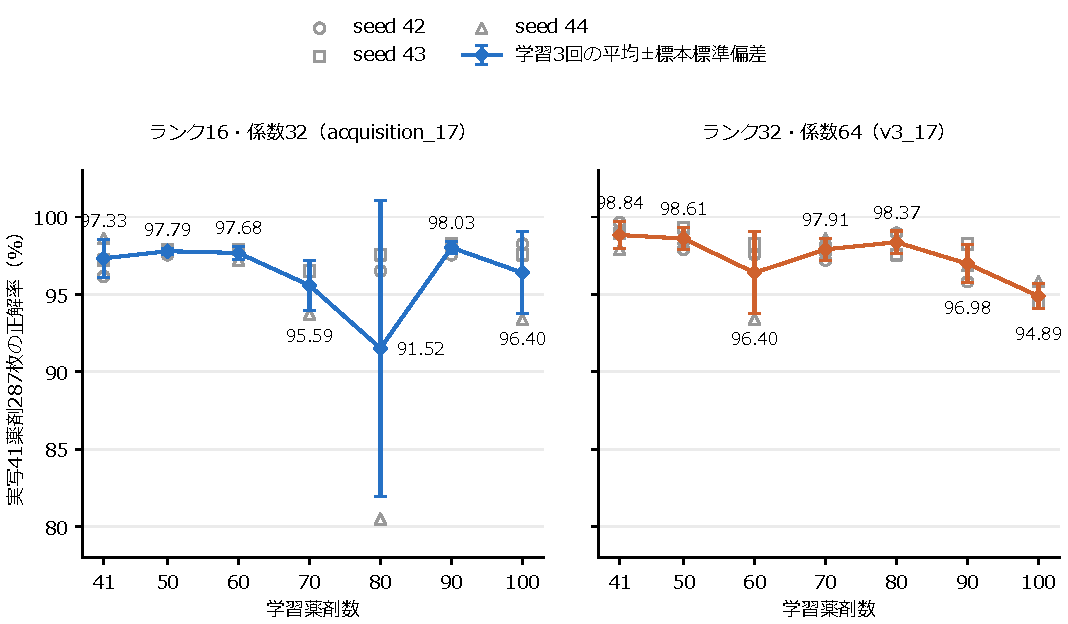
\includegraphics[width=\linewidth]{figures/generated_261006/class_expansion.pdf}
  \caption[学習薬剤数41から100までの全段階と3回の学習の正解率]{学習薬剤数を41から100まで7水準で増やしたときの，ランク16・係数32系列（左）とランク32・係数64系列（右）の内部開発評価画像287枚単剤正解率（3回の学習）．}
  \label{fig:class_expansion_stages}
\end{figure}

崩れが生じる薬剤数は系列によって異なり，「100薬剤で必ず崩れる」といった共通の法則は確認できなかった．
2系列は，LoRA容量と画像拡張セットが同時に異なり，基画像数（1,224枚から2,994枚）と総提示数（107,525枚から262,990枚）も増加した．
したがって，正解率の変化を学習薬剤数だけの効果に分けて説明できなかった．

主結果と同じLoRA容量・拡張セット（ランク16・係数128，\texttt{v3\_17}）で，100薬剤を学習した条件も評価した．
基画像は2,994枚，総提示数は262,990枚であった．
正解数は，乱数シード42が282/287（98.26\%），43が273/287（95.12\%），44が278/287（96.86\%）であり，3回の学習の合計で833/861（96.75\%）であった．
41薬剤のr16\_a128（3回の学習の平均99.54\%）より低かった．
ただし，基画像数と総提示数も異なるため，差を学習薬剤数だけの効果に分けて説明できなかった．
正確McNemar検定を用い，100薬剤を学習したr16\_a128条件を6条件と比較した．
比較対象は，41薬剤のr16\_a128，ランク32・係数64系列とランク16・係数32系列の100薬剤条件，およびGeminiの3条件であった．
6つの比較に合わせて有意とする基準を厳しくした．
100薬剤を学習した条件と41薬剤のr16\_a128の比較は，乱数シード43のみ有意であり（$p=0.0001221$），42と44は有意でなかった（$p=0.21875$，$0.14600$）．
100薬剤を学習した条件の正解率は3回とも41薬剤の条件より低かったが，3回に共通する有意差は確認できなかった．
薬剤が増えると正解率が変わるため，薬剤数を変えるたびに学習の設定を再度調整する必要があると考えた．

\subsection{隙間のない合成複数薬剤画像}\label{sec:zero_gap_top10_results}

薬剤数2，3，5，8の隙間のない元写真タイルを各200枚，合計800枚用いた（固定800枚）．
800枚から抽出された候補は4,336領域であり，期待薬剤ラベル数は3,600であった．
結果の最高値，ver4条件Dの値およびr16\_a128の値を，表\ref{tab:zero_gap_top10_summary}に示す．

\begin{table}[htbp]
  \centering
  \renewcommand{\arraystretch}{1.5}
  \caption{隙間のない合成複数薬剤画像800枚に対するTop-10方式とTop-N方式}
  \label{tab:zero_gap_top10_summary}
  \small
  \setlength{\tabcolsep}{3pt}
  \begin{tabular}{|p{2.6cm}|p{2.1cm}|r|r|>{\raggedright\arraybackslash}p{4.7cm}|}
    \hline
    方式 & \shortstack[l]{最高条件\\（ver1〜ver9）} & \shortstack{最高結果\\（800枚）} & \shortstack{ver4\\条件D} & r16\_a128（3回の学習） \\ \hline
    薬剤数未知・Top-10方式 & ver5-2，ver5-3，ver8 & 790/800（98.75\%） & 76.25\% & 3回とも790/800（98.750\%） \\ \hline
    薬剤数既知・Top-N方式 & ver8 & 682/800（85.25\%） & 66.50\% & \shortstack[l]{学習3回の平均\\85.000\%$\pm$0.125pt} \\ \hline
  \end{tabular}

  \vspace{1mm}
  {\scriptsize Top-10方式は余分な予測を許すため，790/800は画像完全一致率ではなく正解薬剤包含率である．r16\_a128の値は，乱数シード42，43，44のアダプタをRTX 4070 Ti SUPERで実測したものであり，H100の結果との直接比較には用いない．}
\end{table}

Top-10方式では，ver5-2，ver5-3およびver8が同率で790/800（98.75\%）となり，最高であった．
この方式は，正解薬剤を取りこぼさないことを優先し，過検出を罰しない．
Top-N方式は，全条件でTop-10方式を下回り，最高はver8の682/800（85.25\%）であった．
候補の強度順位は，薬剤領域の完全性や識別しやすさを直接表さないため，正しい候補が$N$位より後ろに残ることが低下の一因と考えた．
r16\_a128では，Top-10方式が3回とも790/800（98.750\%）であり，ver1からver9の最高値と一致した．
Top-N方式は，乱数シード42，43，44でそれぞれ681/800，680/800，679/800であり，ver8の682/800を下回った．
r16\_a128のTop-N方式の画像正解率は，薬剤数が増えるほど低下し，2薬剤の96.500\%から8薬剤の64.333\%まで下がった．
Top-10方式では，8薬剤でも95.000\%を維持した．

図\ref{fig:zero_gap_detection_example}に，固定800枚のうち5薬剤と8薬剤の各先頭1枚について，検出された候補枠と採点用の正解タイルを重ねて示す．
検出器へは画像だけを与えた．
2枚は各薬剤数の先頭の画像であり，結果を見て選んだ画像ではない．
薬剤名の予測には，r16\_a128の乱数シード42を用いた．

\begin{figure}[htbp]
  \centering
  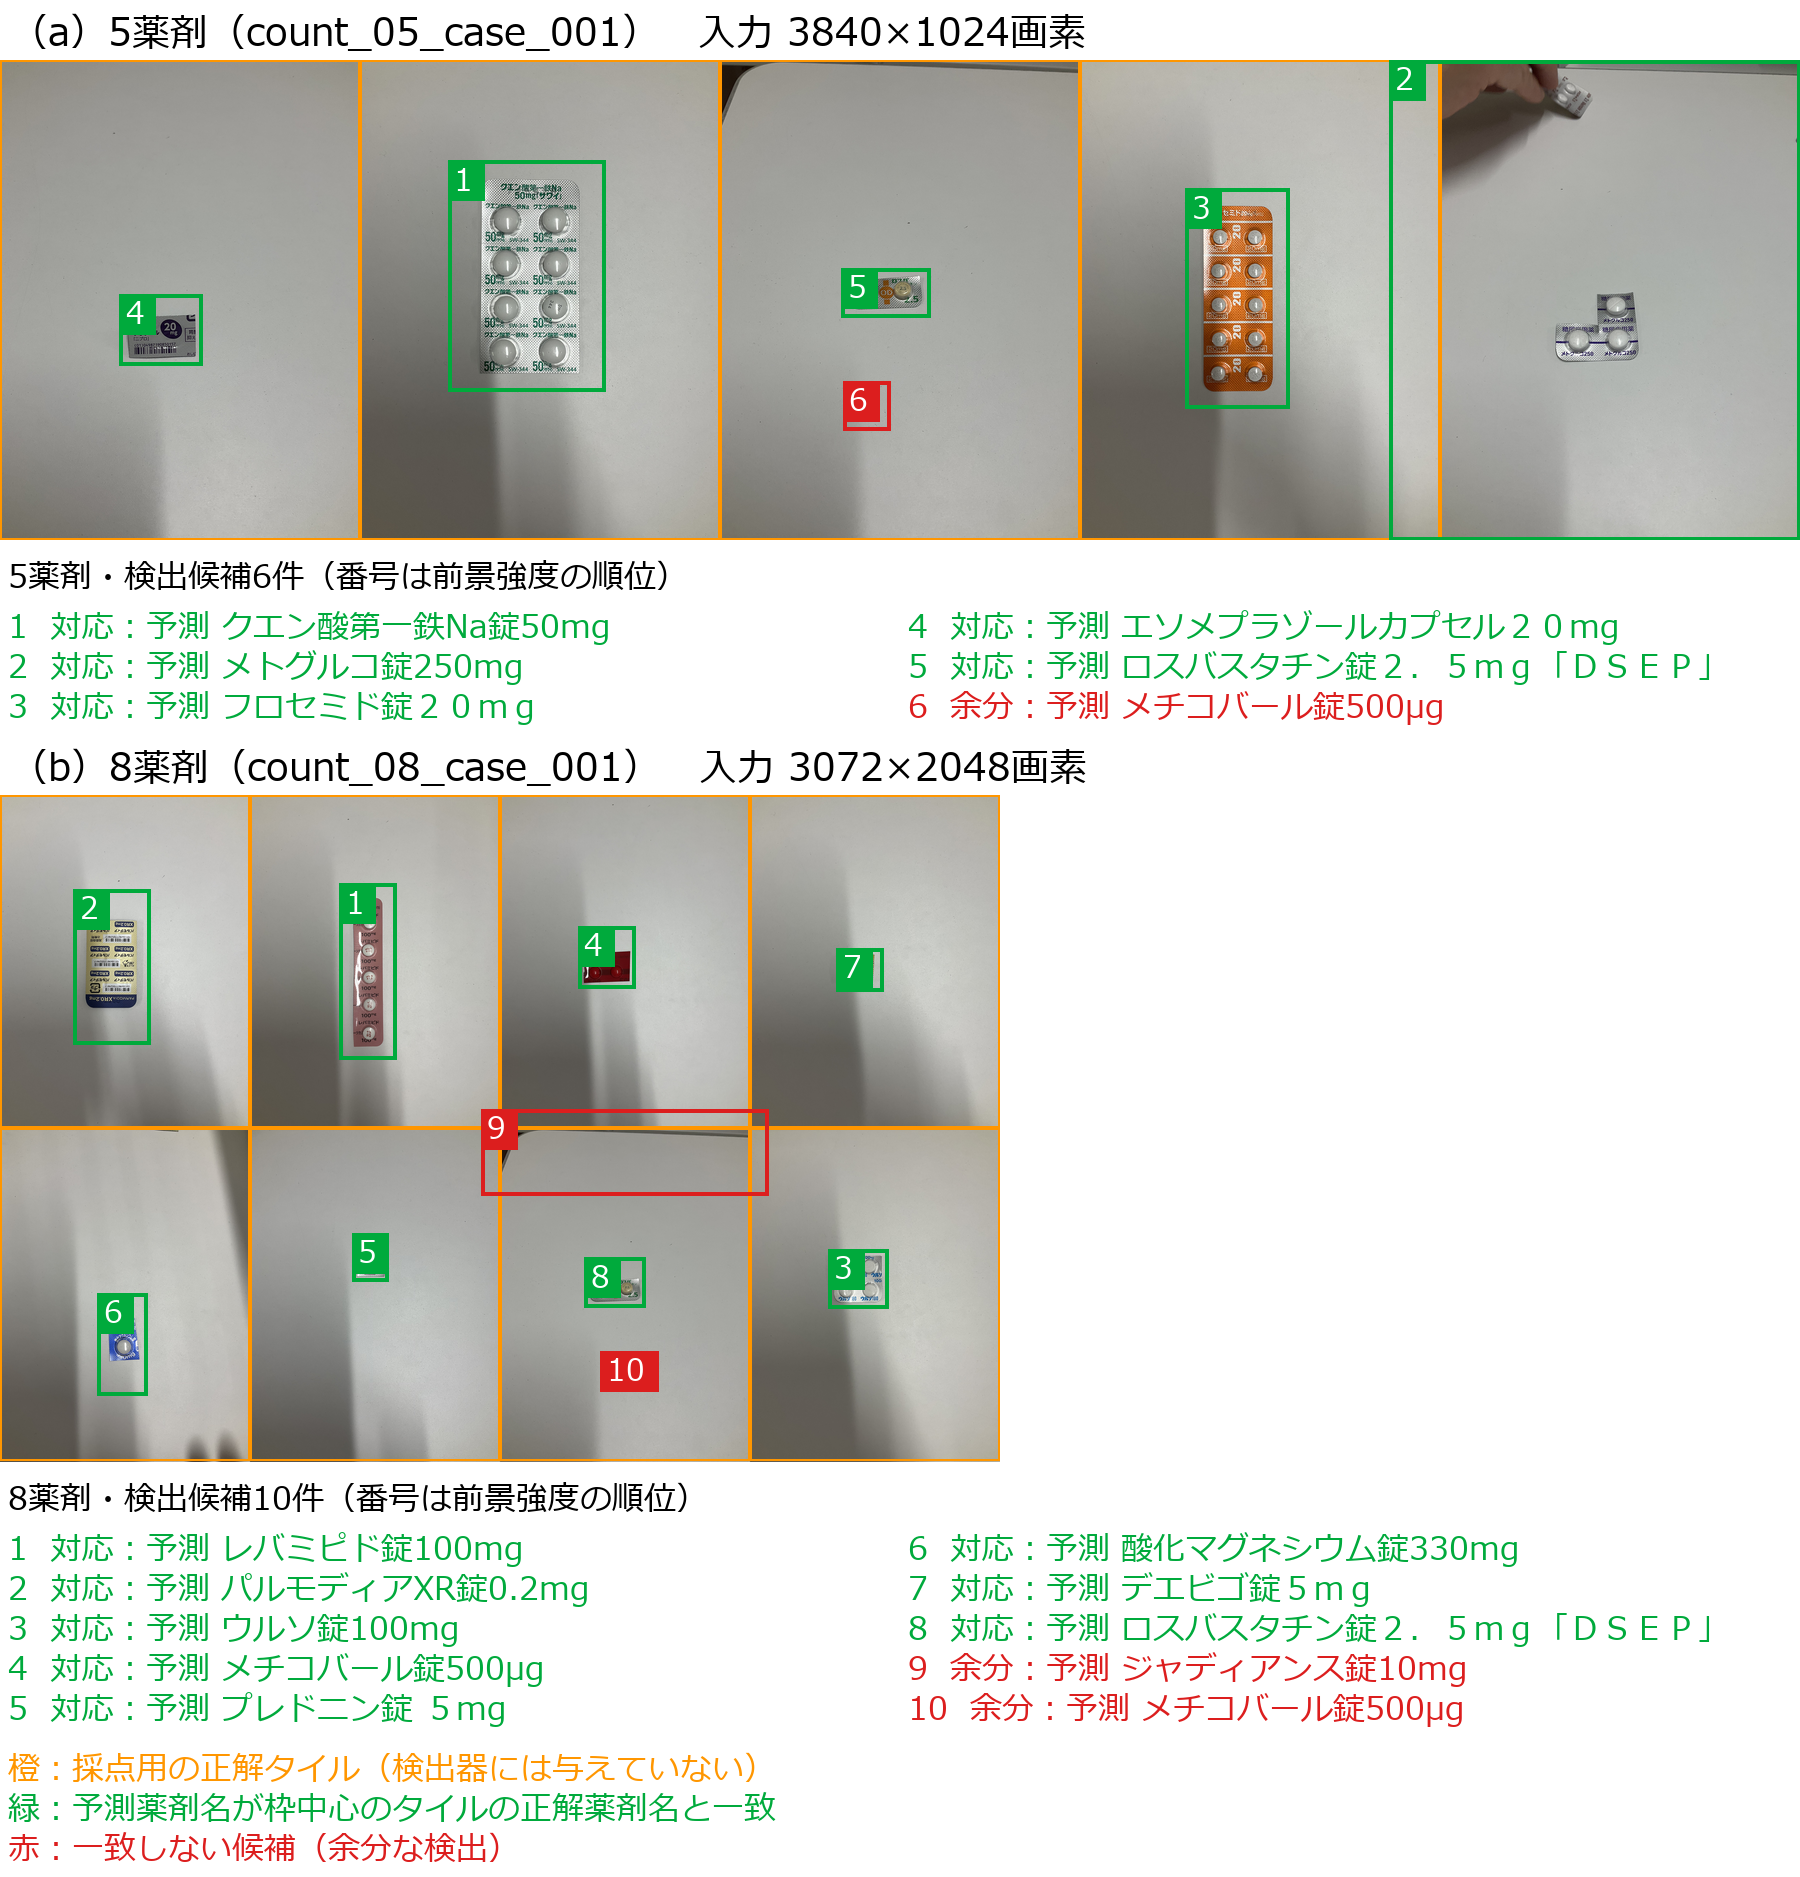
\includegraphics[width=\linewidth]{figures/generated_ver10/zero_gap_fixed800_detection_example.png}
  \caption[固定800枚における検出候補枠と正解タイルの実例]{固定800枚における検出候補枠と正解タイルの実例．（a）は5薬剤，（b）は8薬剤の各先頭1枚である．橙色が採点用の正解タイル，緑色が予測薬剤名と枠中心のタイルの正解薬剤名が一致した候補，赤色が一致しなかった候補である．}
  \label{fig:zero_gap_detection_example}
\end{figure}

5薬剤の画像（同図（a））では6候補が検出され，5候補が各タイルの薬剤と一致した．
残る1候補は，正解薬剤に含まれない薬剤と予測された余分な検出であった．
8薬剤の画像（同図（b））では10候補が検出され，8候補が一致し，2候補が余分であった．
2枚とも，余分な候補は順位$N$より後ろであり，Top-10方式とTop-N方式のいずれでも成功と記録されていた．
一方，余分な候補が正解薬剤の候補より上位に入る画像では，Top-N方式で失敗する．
過検出の影響は画像によって異なった．

\subsection{総合考察}

本報告書が示した単剤正解率は，性質の異なる3つの区分に分かれる．
表\ref{tab:headline}に，その位置付けを示す．

\begin{table}[htbp]
  \centering
  \caption{本報告書が示す単剤正解率の位置付け（内部開発評価画像287枚）}
  \label{tab:headline}
  \small
  \setlength{\tabcolsep}{3pt}
  \begin{tabular}{|p{2.6cm}|p{2.4cm}|p{3.0cm}|p{4.5cm}|}
    \hline
    位置付け & 条件 & 単剤正解率 & 扱い \\ \hline
    主結果 & r16\_a128（3回の学習） & 99.54\%$\pm$0.53pt & 8条件を比較した後に平均正解率が最も高い条件として選んだ．検定した14組では，学習3回に共通する有意差はなかった． \\ \hline
    従来の主結果（別系統） & ver4条件D & 280/287（97.56\%） & 実験の開始前に主結果として定めた設定の，1回学習の観測値であった． \\ \hline
    探索的な最高観測値 & ver6，ver8，ver9 & 286/287（99.65\%） & 結果を確認した後に選んだ条件であり，確認的な主結果ではない． \\ \hline
  \end{tabular}
\end{table}

条件比較では，量子化，LoRAのランク，係数，学習対象層などを同時に変更しており，個別の要因の効果は分離できなかった．
ver6の286/287は，ver4条件Cに対して有意でなかった．
LoRAのランクと係数を変えた8条件について，14組の比較を行った．
検定した14組では，学習3回に共通する有意差は確認できなかった．
ランクを上げると学習するパラメータ数が増える．一方，係数は更新の大きさを変えるものであり，パラメータ数は増えない．その違いから，薬剤数が増えた場合には設定を変える効果が出る可能性があると考えた．
今回は41薬剤と少なかったため，設定を変えた効果が見えにくかった可能性があると考えた．ただし，この理由を確かめる実験は行わなかった．

単剤の主結果r16\_a128は，99.54\%$\pm$0.53pt（3回の学習の平均）であり，従来の主結果ver4条件Dは97.56\%であった．
両者の直接検定は，シードにより判定が割れた．
r16\_a128は8条件の結果を見て選んだ条件であった．
287枚を条件選択と評価の双方に使用しているため，結果を見て条件を選んだ影響が残った．
LoRAなしでは287枚中3枚，追加学習したver4条件Dでは280枚に正解した．
LoRAによる追加学習で，対象薬剤の特徴を学べたためと考えた．
候補一覧を与えたGemini 3.8 Flashとは，41薬剤について有意差のない結果を得た．
候補を与えないGeminiの2条件を有意に上回った．
ただし，候補一覧付きの条件は入力条件が対等でなく，有意差がないことは同等の証明ではない．
本手法は外部のサービスにデータを送らず，手元の計算機で動かせる点に意味があると考えた．

固定800枚では，薬剤数を仮定しないTop-10方式の98.75\%に対し，薬剤数を既知とするTop-N方式の最高は85.25\%であった．
画像単位の完全一致では，候補中の誤りが画像全体の不一致となる．
複数薬剤では，薬剤の領域を切り出す処理の失敗と，正しい候補が$N$位より後ろに残ることが，正解率を下げた原因と考えた．
ただし，それぞれがどれだけ影響したかは分けて確かめなかった．

信頼ゲートは，どちらのモデルでも未知薬剤への危険通過を0件にできなかった．
この点は，未知薬剤の種類を増やして確かめ，誤回答をさらに減らす必要があると考えた．

\subsection{評価範囲と注意点}

今回の評価の範囲と，結果を解釈する際の注意点を以下に示す．

\begin{enumerate}
\setlength{\itemsep}{0pt}
  \item 評価対象は41薬剤に限られた．収集画像のうち10ファイルは，収集時の元ファイルからの加工履歴をたどれなかった．
  \item 評価に用いた287枚は条件検討に反復使用しており，条件を決めた後に別の写真で確認する評価は行わなかった．r16\_a128も8条件を同じ287枚で比較した後に選んだため，結果を見て条件を選んだ影響が残った．
  \item 主結果は3回の学習（乱数シード42，43，44）で評価したが，ver1からver9，ver4条件Dや信頼ゲートなど一部の比較は1回の学習であった．これらの比較では学習のばらつきを評価しなかった．McNemar検定では画像対の独立性を確認できず，複数比較の補正は，問いごとに14組，3組，6組の範囲で行った．
  \item 固定800枚はタイル合成画像であり，実写の複数薬剤画像での性能は確かめなかった．また，信頼ゲートはver4条件Dとver6だけに適用し，既知側と未知側の撮影条件も異なった．
  \item LoRAなしとの比較はver4条件Dとの比較であり，Geminiの候補一覧付き条件とは入力条件が異なった．短文条件では同じ画像と同じプロンプトを用いた．画像分類器との比較は行わなかった．
  \item CUDAの決定論的アルゴリズムを無効にしており，ビット単位の再現は保証されない．収集画像の整理や撮影に要した時間と，スマートフォン上の動作は評価しなかった．
\end{enumerate}

%----------------------------------------------------------------------
\clearpage
\section{結論・今後の課題}\label{sec:conclusion}
%----------------------------------------------------------------------

\subsection{結論}

本研究の目的は，1薬剤当たりフルシートの表面画像1枚と裏面画像1枚から学習集合を構成し，41薬剤のPTP包装識別性能を評価することであった．
この目的に対し，収集した表裏のフルシート画像からRTIと部分画像を生成した．
主結果の条件では，RTIを学習に含めず，全体画像と部分画像を用いた．
続いて，画像拡張を適用し，Qwen3.5-4BをLoRAで追加学習した．
大学病院薬剤部で撮影した内部開発評価画像287枚を用いて，単剤正解率を評価した．

単剤の主結果として採用したr16\_a128は，3回の学習の平均で99.54\%（標本標準偏差0.53pt，286/287，287/287，284/287）であった．
ただしr16\_a128は，LoRA容量を変えた8条件の中で平均が最も高かった条件であった．
検定した14組では，学習3回に共通する有意差は確認できなかった．
同じ評価画像で条件を選んだ影響は残った．
従来の主結果であるver4条件Dは280/287（97.56\%）であり，r16\_a128との直接検定はシードにより判定が割れた．
LoRAなしのQwen3.5-4Bは3/287であり，ver4条件Dとの差は有意であった．
Geminiとの比較では，短文条件を3回とも有意に上回ったが，候補一覧付きの条件とは有意差がなかった．
固定800枚では，Top-10方式が最高790/800（98.75\%），Top-N方式が最高682/800（85.25\%）であった．
信頼ゲートは，ver4条件Dで4/58，ver6で2/58の未知薬剤への危険通過があり，0件にできなかった．
学習薬剤数を41から100へ増やしても，既知41薬剤の正解率は単調に変化しなかった．

LoRAによる追加学習で正解率が上がったのは，対象薬剤の特徴を学べたためと考えた．
一方，ランクや係数を比較した範囲では，学習3回に共通する有意差は確認できなかった．
学習した薬剤数が41と少なかったことが，効果の見えにくさに関係した可能性があると考えた．
複数薬剤では，薬剤の領域を切り出す処理の失敗と，正しい候補が$N$位より後ろに残ることが，正解率が低くなる原因と考えた．
学習薬剤数を変えると正解率が変わるため，再度の調整が必要と考えた．

各薬剤の表面1枚と裏面1枚から学習画像を生成し，今回の41薬剤のPTP包装を識別できることを確認した．
一方，実写の複数薬剤画像での評価や作業負担の測定は行わず，未知薬剤への誤回答も残った．

専用の撮影機材を使わず，少ない収集画像でモデルを学習できた．
このモデルは，候補一覧を与えたGemini 3.8 Flashと有意差のない正解率を示した．
また，手元の計算機で動かせた．
外部にデータを出したくない場面で使える点に意義があると考えた．
ただし，作業時間の削減は測定しなかった．

\subsection{今後の課題}

第一の課題は，学習する薬剤の数を増やしても正解率を保つことであった．追加した薬剤については，学習に使わない実写画像での評価が残った．
第二の課題は，部分画像の内容と学習量のどちらが結果に効いたかを調べることであった．学習量をそろえて画像の組合せを変える比較と，複数回の学習による確認が残った．

その次に，未知薬剤への回答保留と，実写の複数薬剤画像での識別が課題となった．未知薬剤では，既知薬剤と同じ撮影条件で誤回答を減らせるかが未確認であった．

\clearpage

\section*{謝辞}
\addcontentsline{toc}{section}{謝辞}

本研究の遂行にあたり，多大なご指導とご助言を賜った森山真光准教授に，心より感謝する．
また，本研究で用いた薬剤画像の撮影にご協力いただくとともに，薬剤鑑別に関する貴重なご助言を賜った共同研究者である近畿大学病院薬剤部の皆様，ならびに木村裕一教授に深く感謝する．

\clearpage
\addcontentsline{toc}{section}{参考文献}

{\footnotesize
\raggedright
\bibliographystyle{junsrt}
\bibliography{261006}
}

\end{document}
